%!TEX TS-program = pdflatex                                                    %
%!TEX encoding = UTF8                                                          %
%!TEX spellcheck = en-US                                                       %
%------------------------------------------------------------------------------%
% to compile use "latexmk --pdf main.tex"                                      %
%------------------------------------------------------------------------------%
% to count words 
% "pdftotext main_nofigs_nocaptions.pdf - | egrep -e '\w\w\w+' | iconv -f ISO-8859-15 -t UTF-8 | wc -w"
% -----------------------------------------------------------------------------%

\documentclass{bioinfo}
\usepackage{url}
\usepackage[english]{babel}
\usepackage[utf8]{inputenc}
\usepackage[T1]{fontenc}
%\usepackage[pdftex]{graphicx} 
%\usepackage{graphics}
%\usepackage{hyperref}
\usepackage{float}
\floatplacement{figure}{H}
\usepackage{booktabs}     % nice tables
\usepackage{tabularx}     % even nicer tabular environments 
\usepackage{amsmath}
\usepackage{amsfonts}
\usepackage{amssymb}
%\usepackage{multicol}
\usepackage{listings}
\usepackage{tikz,times}
\usepackage{courier}
\usepackage[scaled]{beramono}

\usetikzlibrary{shapes,arrows}
\usetikzlibrary{arrows,positioning}
\usepackage{xcolor}
\usepackage[font=bf]{subfig}
\usepackage[inline]{trackchanges}

%%%%%%% setup track changes "editors"

\addeditor{mw}
\addeditor{lp}
\addeditor{psl}
\addeditor{ld}
\addeditor{vj}
\addeditor{sk}
\addeditor{jm}

%\usepackage{sectsty}
%\sectionfont{\normalsize\bfseries}
%\usepackage[labelfont=bf]{caption}
%\usepackage{endfloat} %place figures at end of document
%------------------------------------------------------------------------------%
%\captionsetup{
%%format = hang,                % caption format
%labelformat = simple,          % caption label : name and number
%labelsep = period,             % separation between label and text
%textformat = simple,           % caption text as it is
%justification = justified,     % caption text justified
%singlelinecheck = true,        % for single line caption text is centered
%font = {up,singlespacing},     % defines caption (label & text) font
%labelfont = {bf,footnotesize}, % NOTE: tiny size is not working
%textfont = footnotesize,
%%width = \textwidth,           % define width of the caption text
%skip = 1ex,                    % skip the space between float and caption
%listformat = simple,           % in the list of floats, label + caption
%}

%------------------------------------------------------------------------------%
%\hypersetup{
%    bookmarks=true,         % show bookmarks bar?
%    unicode=false,          % non-Latin characters in Acrobat’s bookmarks
%    pdftoolbar=true,        % show Acrobat’s toolbar?
%    pdfmenubar=true,        % show Acrobat’s menu?
%    pdffitwindow=false,     % window fit to page when opened
%    pdfstartview={FitH},    % fits the width of the page to the window
%    pdftitle={TheVirtualBain},    % title
%    pdfauthor={PSL},        % author
%    pdfsubject={ProposedArticle},   % subject of the document
%    pdfcreator={paupau},    % creator of the document
%    pdfnewwindow=true,      % links in new window
%    colorlinks=true,       % false: boxed links; true: colored links
%    linkcolor=red,          % color of internal links (change box color with linkbordercolor)
%    citecolor=blue,        % color of links to bibliography
%    filecolor=magenta,      % color of file links
%    urlcolor=blue           % color of external links
%}
%-----------------------------------------------------------------------
%\usepackage{subcaption}

%%%%%%%%%%%%%%%%%%%%%%%%%%%%%%%%%%%%%%%%%%%%%%%%%%%%%%%%%%%%%%%%%%%%%%%%%%%%%%%%
%%                             New and renew commands                         %%
%%%%%%%%%%%%%%%%%%%%%%%%%%%%%%%%%%%%%%%%%%%%%%%%%%%%%%%%%%%%%%%%%%%%%%%%%%%%%%%%
  
\renewcommand{\lstlistingname}{Code}
\renewcommand{\thesubfigure}{\Alph{subfigure}}
%\newcommand{\inputTikZ}[2]{\scalebox{#1}{\input{#2}}}
\newcommand*{\h}{\hspace{5pt}}   % for indentation
\newcommand*{\hh}{\h\h}          % double indentation
\newcommand{\TVB}{\textit{TheVirtualBrain }}
\newcommand*{\tvbmodule}[1]{{\textsc{#1}}}          % scientific modules in "simulator"
\newcommand*{\tvbdatatype}[1]{\textbf{\emph{#1}}}   % datatypes in "datatypes"
\newcommand*{\tvbclass}[1]{{\ttfamily\emph{#1}}}    % classes either in simulator mods or datatypes
\newcommand*{\tvbmethod}[1]{{\textsf{#1}}}          % methods
\newcommand*{\tvbattribute}[1]{{\ttfamily{#1}}}     % attributes
\newcommand*{\tvbtrait}[1]{{\ttfamily{#1}}}         % traited types



%%%%%%%%%%%%%%%%%%%%%%%%%%%%%%%%%%%%%%%%%%%%%%%%%%%%%%%%%%%%%%%%%%%%%%%%%%%%%%%%
%%                            Colors and graphics                             %%
%%%%%%%%%%%%%%%%%%%%%%%%%%%%%%%%%%%%%%%%%%%%%%%%%%%%%%%%%%%%%%%%%%%%%%%%%%%%%%%%
\definecolor{palegreen}{HTML}{DAFFDA}
\definecolor{lightgray}{rgb}{0.15,0.15,0.15}
\definecolor{orange}{HTML}{FF7300}
\DeclareGraphicsExtensions{.jpg,.pdf,.png,.tiff}%,.mps,.bmp
\graphicspath{{figures/}}
 
%##--------------------------------------------------------------------------##%
%##                               START HERE                                 ##%
%##--------------------------------------------------------------------------##%
\copyrightyear{}
\pubyear{}

\begin{document}
\lstset{language=Python,
	captionpos=b,
	keepspaces=true,
	numbers=none,
	showspaces=false,
	basicstyle=\fontsize{8pt}{8}\ttfamily
	} 

\firstpage{1}

%%  Authorship and Title
\title[TVB]{Integrating neuroinformatics tools in TheVirtualBrain}
\author[Woodman {et~al}]{
        M. Marmaduke Woodman\,$^{1,*}$,  
        Laurent Pezard\,$^{1,*}$,  
        Lia Domide\,$^{3}$, 
        Stuart Knock\,$^{1}$, 
        Paula Sanz Leon\,$^{1}$, 
        Jochen Mersmann\,$^{2}$,
        Anthony R. McIntosh \,$^{4}$ and  
        Viktor Jirsa\,$^{1}$\footnote{to whom correspondence should be addressed: marmaduke.woodman@univ-amu.fr,
        viktor.jirsa@univ-amu.fr}}

\address{$^{1}$ Institut de Neurosciences des Syst{\`e}mes, 27, Bd. Jean Moulin, 13005, Marseille, France.\\
         $^{3}$ Codemart, 13, Petofi Sandor, 400610, Cluj-Napoca, Romania.\\
         $^{2}$ CodeBox GmbH, Hugo Eckener Str. 7, 70184 Stuttgart, Germany.\\
         $^{4}$ Rotman Research Institute at Baycrest, Toronto, M6A 2E1, Ontario, Canada\\
        }

\history{}

\editor{}

\maketitle

%##--------------------------------------------------------------------------##%
%##                               ABSTRACT                                   ##%
%##--------------------------------------------------------------------------##%


\begin{abstract}
\section{}

TheVirtualBrain (TVB) is a neuroinformatics Python package representing the
convergence of lines of work in clinical, systems, theoretical neuroscience in
the integration, analysis, visualization and modeling of neural dynamics of the
human brain as well as the imaging modalities through which these dynamics are
measured. Specifically, TVB is composed of a flexible simulator for both neural
dynamics and modalities such as MEG and fMRI, common analysis techniques such
as wavelet decomposition and multiscale sample entropy, interactive visualizers
for replaying cortical timeseries on the 3D surface or editing large-scale
connectivity matrices, and an (optional) user interface accessible through
modern web browsers. Tying together these pieces with persistent data storage,
based on a combination of SQL \& HDF5, is a rich, open-ended system of
datatypes modeling (systems level) neuroscientific data and the relations among
them. This data modeling system in parallel with the so-called adapter pattern
architecture permit the integration of TVB with any other computational system,
including MATLAB for which support is already available.  Notably, TVB provides
infrastructure for multiple projects and multiple users, possibly participating
under multiple roles: a clinician may import diffusion spectrum imaging data,
launch a tractography algorithm, and identify potential lesion points, and then
share this data with a computational expert who would then enter to contribute
simulation parameter sweeps and analyses, to test which lesion point is most
probably given certain empirical imaging data, et cetera; this is one of many
multi-user use cases supported by TVB.  TVB also drives research forward on
many levels: the simulator itself represents the systematization of several
recent ad-hoc simulations in the modeling literature on human rest state.  In
these ways, TVB serves as an integrating platform for disparate expertises in
the high level analysis and modeling of the human brain.  This paper will begin
with a brief outline of the history and motivation for TVB as a unified project
\textit{per se}. We proceed to describe the framework and simulator, giving
usage examples in the web UI and in plain Python scripting.  Finally, we
compare TVB with the nearest neighbors in brain modeling, simulation
performance, recent advances thereupon with native code compilation and GPUs,
and the role of Python and its rich scientific ecosystem in TVB. 

  
\section{Keywords:} connectivity, connectome, neural mass, neural field, 
time delays, full-brain network model, Python, virtual brain, large-scale 
simulation,  web platform, GPUs
\end{abstract}

\section{Motivation}
The advancement of neuroscience and more generally brain and behavioral sciences require
significant interaction between scientific disciplines in order to fulfill their goal
of understanding the relationship between brain and cognition\footnote{Several
important scientific projects such as The Human Brain Project are clear
illustration of this.}. Nevertheless, one major drawback of this
interdisciplinary enterprise is the necessary distribution of competences, most
frequently between individuals but also, in a non negligible number of cases,
between institutes.  Moreover, the technicalities involved in data
analysis and brain simulation usually prevents an optimal diffusion of these
advances to the more experimentally oriented part of the community. 

These problems invite at least two approaches to their solution. Firstly,  the
development of up to date and accessible software libraries developed in commonly
used programming languages and secondly, the development of tools for sharing
competences and data. Due to the high pace of new developments, these solutions
should also remain open to incoming new tools. Several projects fall in the
first category (from SPM to connectivity toolbox, fieldtrip in the \matlab{} ``galaxy''
and from ``nitime'' to neo... to name only a few). In the second category CARMEN
(http://www.carmen.org.uk/) and G-Node (https://portal.g-node.org/data/)
\note[lp]{Other projects?} are (web) platforms for collaborative work and data
sharing. The diffusion of \matlab{} and its integrated environment also usually
take place of the platform / development environment. 
\note[sk]{not exactly sure what this last sentence is trying to say, so, needs rewording}

TheVirtualBrain (TVB) provides its own solutions to these two problems.  In an
initial step, these two problems were addressed in two independent projects: one
whole brain-simulator library developed in \matlab{} and a web platform for
collaborative interactions in the context of multi-purpose data analysis which
was developed in Python.  In each case, the choice of the language was dictated
both by the scientific context and the technical constraints. The whole brain
simulation library was developed in \matlab{} due to the \note[lp]{unfortunate}
widespread use of the language in the neuroscientific community. On the
other hand, the platform was designed for a more generic purpose, such as providing several
interfaces for user interaction (web and console) and the capability to adapt
to existing and future libraries. In this latter case, the programming language
should adapt to tasks from  web development to numerical methods implementation
and should be able to act as a ``glue'' language. These constraints
\note[lp]{naturally} oriented the development of the framework toward
Python\footnote{The first issue of Python in Neurosciences also confirmed the
choice of the Python language.}.  Moreover, Python is a language that provides
the main blocks needed for the project: database interactions, web programming,
object-oriented programming and abstraction. \emph{TheVirtualBrain} benefits
from this initial development which remain in the overall organization of TVB's
architecture: the \emph{framework} and the \emph{scientific library}.

\note[sk]{Terminology (consistency with usage in code naming, docs, previous publications):
          Architecture => overall design (think whitepaper and Lia's diagrams of TVB's architecture;
          Framework => the specific component/package covering database back-end, 
            web interface, etc...)}

\subsection{Why another project? (TVB compared to others)}

The reasons for developing a new project are different for each component of
TVB.

\subsubsection{The framework}
\note[sk]{this subsubsec repeats itself a bit, rearrange existing into 2 paras,
ideally incorporating any comment Lia makes re lp's note}

In effect, we wish for a theoretician and a more experimentally-oriented
neuroscientist to be able to collaborate; to enable such a possibility, we
require a platform that simultaneously provides power, flexibility, and a 
simple interface.
To address these concerns, a flexible architecture was developed to
allow easy integration of any computational tools along with a system
for describing typical types of data. A web based UI was developed
for users not comfortable with programming.
% as well as \matlab{} toolbox for interacting with the Python based framework,
% given that many neuroscientists are already comfortable with the \matlab{}
% workflow.

The two main constraints for the architecture were then to provide a web
interface to allow remote collaboration and a data exchange system to allow the
exchange of data (experimental or simulated) between scientists. To this end,
the particular design chosen for TVB's architecture was the well-known
``model-view-controller'' pattern \note[lp]{detail this}. Initially, an attempt 
was made to develop the architecture using an existing integrated / high-level web
framework, but we rapidly found ourselves struggling with the implementation, using
a framework that did not fit our needs. Due to the availability of a wide range of
Python Packages, we then choose to use more specific blocks for each purpose and
build the necessary interaction between them ourselves. For this purpose, we choose
\textsf{CherryPy} for the web  and \textsf{SQLAlchemy} for the database
exchanges\footnote{Other dependencies of TVB are listed in
    \texttt{TVB\_INSTALL\_REQUIREMENTS} which currently lists
    \texttt{"apscheduler", "beautifulsoup", "cherrypy", "cfflib", "formencode",
        "lxml", "minixsv", "mod\_pywebsocket", "networkx", "nibabel", "numpy",
        "numexpr", "psutil", "scikit-learn", "scipy", "simplejson",
        "sqlalchemy", "sqlalchemy-migrate"}.}

In addition to this, to fulfill the requirement of 3D data visualization, we 
made use of the availability of WebGL in modern browsers.

The architecture of TVB had been prototyped in Python, and in turn, both the
language and the scientific ecosystem were more than rich enough to support
continued developed entirely within Python, of both the framework and the
simulator, in addition to it being a general purpose language. Lastly, Python's
emphasis on readability and idiomatic style facilitates integration of 
code contributions from programmers with disparate backgrounds.

\note[lp]{For Lia: Was Python a "good" choice? and why? Which other language would have
done the job?}

\subsubsection{The simulator}

In the case of the simulator, the situation was a little different, 
a set of \matlab{} routines had been developed that did the job but were never
intended for generic
deployment. The choice was between: develop our own simulator by porting the 
existing \matlab{} routines to Python and a more generic structure, or make use
of an existing simulation library. As in the case of the framework, we started 
by trying to use an existing
simulator, namely Brian \cite{Goodman_2009} since it has a very generic way of
specifying models by differential equation expressions. Although we had some
success in the implementation of several models in Brian we found ourselves in a
similar situation to that with the framework, having to hack around incompatibilities
between the purpose for which the Brian was designed and our goals. 

In fact, the core simulator began in \matlab{}, however, as the needs 
expanded, the framework quickly 
outgrew the matrix-struct-function triumvirate that is conventional
in \matlab{} programming. While modern \matlab{} permits advanced object-oriented
programming, it has the disadvantages of being relatively unused, and
largely unsupported by \matlab{}'s own IDE, the \matlab{} Compiler, and the free
alternative Octave, lastly it provides no support for metaclasses or data
descriptors, which were extensively used in TVB's architecture.

The major constraints came from the scale of the simulation in TVB that is
clearly different from the more usual ``cellular'' simulations. One needs specific
population / field models and moreover should produce simulated experimental
data at macroscopic levels such as EEG, MEEG and fMRI which are not usually
simulated in the current neuronal simulators.

Although the scale of simulation is clearly different and imply specific
orientations for TVB simulator, the overall structure of neural model remains
and we happen to borrow concepts such as \emph{monitors} (which are objects that
record the course of a simulation) from Brian but
implement them in the context of TVB simulations.


While whole-brain level simulators have been developed and published for
several years now, making the final step of connecting these simulations to
empirical results has remained a challenge due to several factors:

\begin{enumerate}

	\item Source code is typically not distributed, effectively closing
        the behavior, black box, etc. \note[lp]{Is this really true for NEURON,
        GENESIS and others? I doubt...}

	\item The forward solutions required to obtain simulated M/EEG \& fMRI
	data are non trivial, requiring interaction with several pieces of software

	\item Published simulation methods for stochastic, delayed systems 
		are almost non existent (XPPAUT \cite{XPPAUT} is a notable exception).
		Efficient handling of $N^2$ delays requires custom routines.

	\item Managing all of the different computational pieces is typically
	challenging for those who work with empirical data.

\end{enumerate}

A significant part of TVB is simulating brain-scale neural networks. While
several existing simulators could have been adapted, we have estimated that
TVB style simulations are far enough outside the design of other simulators to
make starting from scratch a better idea.

Many neural network simulators have been developed and published, focusing
first on abstract rate neurons (in the style of PDP), modelling neurocognitive
processes, on one hand, and on the other, full multicompartmental neuron
simulators treating complex spatial geometries, e.g. NEURON \cite{Hines_2001}.
More recently, due to interest in the computational properties of spiking 
neurons and their relevance to experimental observations, simulators targeting
specifically spiking neurons have been prominent, e.g. Brian 
\cite{Goodman_2009}.

However, another level description of neural dynamics has been treated
in the literature of neural mass models and neural fields 
\cite{Deco_2008a, Coombes_2010}. Here, the spatial
extent of the modeled dynamics is far larger and hence permits networks 
thereof to scale reasonably to the entire cortex, under the assumptions 
of the models, when combined with empirical measurements of cortico-
cortical connectivity. Therefore, the physical scale modeled by the TVB
simulators differs from that for which other simulators were designed.
Several technical issues stem from this scale, e.g. efficient handling
of dense $N^2$ delays and neural field-like connectivity, which will be
discussed in more detail below. 

%Other simulators compared to TVB

	Brian should be a particular focus in this section, as it may
    be one of the closest.  \note[lp]{Dana also (but is it alive?)
    (http://dana.loria.fr/index.html)}

Large scale simulation implies flexible integration. We shall see
how this is enable by the architecture..
\note[mw]{expand}

\subsection{Practical informations / contributors information}

To address these concerns, a flexible architecture was developed to
allow easy integration of any computational tools along with a system
for describing typically types of data. A web based UI was developed
for users not comfortable with programming, as well as \matlab{} toolbox
for interacting with the Python based framework, given that many
neuroscientists are already comfortable with the \matlab{} workflow.

Lastly, a high performance, highly documented simulator along with
various forward solutions have been implemented and released under a
GPL licence to ensure universal access to high quality simulations, 
developed on the well-known Github, making it extremely easy for 
anyone to contribute.

TVB source code is available for download on Github at
\url{https://github.com/the-virtual-brain/}.  Previous Git and Python knowledge
is required for contributing.  Although you could independently install Python
and the rest of TVB dependencies on your machine, and then use the Github code
as a simple local clone, we recommend you to download \emph{TVB\_ Distribution}
from \url{http://www.thevirtualbrain.org/register/}, fork our repositories on
Github and further use \emph{contributor\_setup} script, from inside \emph{TVB\_Distribution} 
folder, to link the two.  In this recommended use-case, you will
have all TVB dependencies already prepared and at your disposal, as part of
\emph{TVB\_Distribution}.\note[lp]{Is there any plan for a .deb package with
full dependencies taken into account in this context? Or Pypi?} 

\note[lp]{Generic description and goal of the paper}

The overall structure of TVB is depitcted on Figure~\ref{fig:architecture} where
components of the architecture and of the scientific library are shown with
their relationships.

 \begin{figure*}
        \centering
        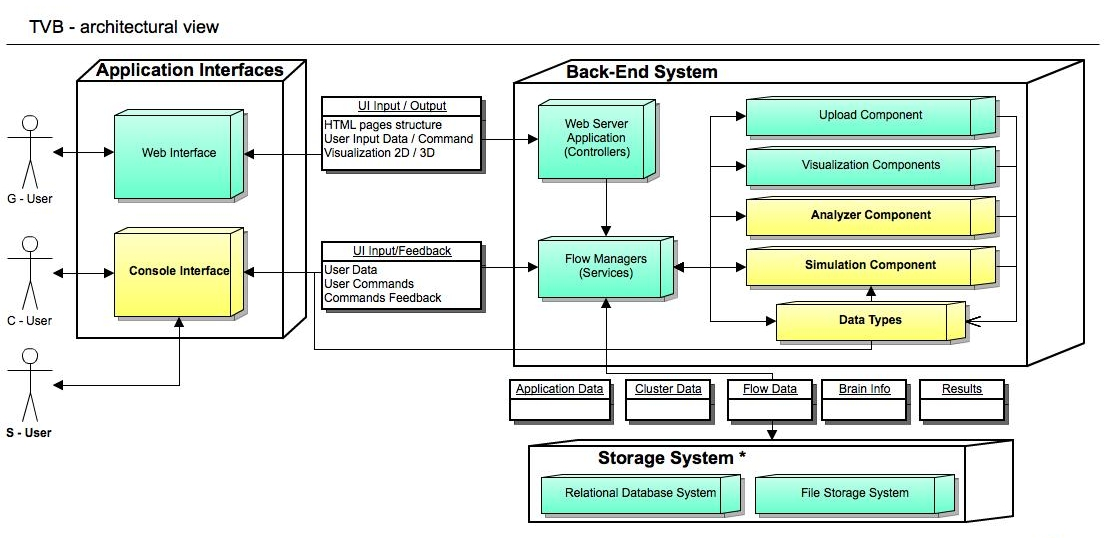
\includegraphics[width=0.90\textwidth]{images/architecture.jpg}
        \caption{TVB architecture: Yellow blocks are part of the Scientific
            Library of TVB, while the green blocks are part of TVB Framework.
            TVB provides two independent interfaces, depending on the
            interaction type wanted by the end-user (web or console).  TVB
            Storage layer is compulsory for the web interface, but it can be
            switched on/off for the console interface.  \note[lp]{It is said in
                the text that "console interface" is part of the "architecture"
            and not the "scientific library", this is the contrary on the
        figure}
        \note[lp]{What is a "S-User"? I missed the definition?}
         }
        \label{fig:architecture}
 \end{figure*}

 The goal of this article is firstly to decribre TVB framework from the
 development point of view and demonstrates how it interacts with other tools
 and how it can be extended (on the basis of extension already integrated in
 TVB).


\section{Architecture}
TVB is logically and technically divided at deploy time into a scientific
library and a framework package, where the scientific library includes
datatypes, basic analyses and the simulator as its central piece, while the
framework handles execution infrastructure, the web-based user interface and
data storage.  TVB Scientific Library can function independently, as a Python
module, but TVB Framework needs to wrap around the scientific library at
runtime. \note[lp]{How is it possible to add extensions to the current version
of TVB?}


\subsection{Basic Concepts}

TVB has been developed with generality and modularity in mind. The central idea
is data-oriented, in the sense that data is fed into and stored in the system,
and can be transformed into another type of data (including visualizations) 
through operations provided by external libraries (including TVB scientific 
library, but not restricted to it) that have been \emph{adapted} to the 
framework. As a consequence, the two central concepts in TVB are: 
\emph{datatypes}, i.e. types of data that can be handled in the framework; and
\emph{adapters}, i.e. classes that allow for the interface/adaption of external
libraries to the datatypes handled within the framework.

TVB framework provides a storage back-end, workflow management and a number of
features to support collaborative work. The framework supports two user 
interfaces: web-based graphical interface and the console interface for 
advanced users and developers.

Due to the generality of the framework, it relies on the Python \emph{abstract classes} mechanism.
\note[lp]{From Python glossary:}
Abstract base classes complement duck-typing by providing a way to define
interfaces when other techniques like hasattr() would be clumsy or subtly wrong.
   
%\begin{verbatim}
%    def configure(self, **kwargs):
%        To be implemented in each Adapter that requires any specific configurations
%        before the actual launch.
%
%    def get_input_tree(self):
%        Describes inputs and outputs of the launch method.
%
%    def get_output(self):
%        Describes inputs and outputs of the launch method.
%
%    def get_required_memory_size(self, **kwargs):
%        Abstract method to be implemented in each adapter. Should return the required memory
%        for launching the adapter.
%
%    def get_required_disk_size(self, **kwargs):
%        Abstract method to be implemented in each adapter. Should return the required memory
%        for launching the adapter in kilo-Bytes.
%
%    def get_execution_time_approximation(self, **kwargs):
%        Method should approximate based on input arguments, the time it will take for the operation 
%        to finish (in seconds).
%
%    def launch(self):
%         To be implemented in each Adapter.
%         Will contain the logic of the Adapter.
%         Any returned DataType will be stored in DB, by the Framework.
%\end{verbatim}


\subsection{Data: types and storage}


\note[lp]{datatypes were first defined in the "architecture" why did it moved to
the scientific library?}
\note[lp]{Is there an "abstract datatype" defined? What is the process to add
new datatype?}

	\subsubsection{TVB Traits}

TVB's traiting system is inspired by the traiting module developed by Enthought \cite{EnthoughtTraits}.
Our traiting system offers a way to annotate fields and classes from inside TVB, with specific trait-attributes,
which will be further used in different layers of the application.
Trait-attributes are synonymous with meta-data for TVB classes and their fields.

\note[sk]{merge the paras above and below this note into one...}

An explicit goal of TVB was to provide a user interface to each of the entities
and algorithms contained within, to achieve this it is necessary at some point to
provide metadata on how to build that interface. To this end, a \texttt{traits}
system was developed, similar to that of IPython or EPD, allowing for attributes
of a TVB class to be written out with full metadata. An extensive set of building 
blocks are already implements from numeric types and arrays to lists, tuples, 
string, and dictionaries.

When methods for a class with annotated fields are invoked, they may use the 
traited-attributes directly, accessing either a default value
or one given during the instantiation of the object. Additionally, this allows
the web-based user interface to introspect a class for all of its fields and their
descriptions, to provide help and choose the proper display form. The explicit typing also allows
such classes to be nearly automatically mapped to storage tables,
thus providing smooth persistence, when the storage layer is enabled.  
Lastly, because such metadata is used to build the docstring of a class,
the IPython user may obtain extensive descriptions of class fields, methods and
arguments in the usual way. 

\note[sk]{merge the paras above and below this note into one...}

So, we have trait-attributes for describing how a certain class with its fields 
will be stored in the database and the file-storage system,
for describing the manner of display in the web-interface, for documenting fields or classes, 
and even providing meta-data on what valid values are allowed on a certain field. 
The complete list of currently supported traited-attributes is described in Table \ref{tab:traits}.

\begin{center}
	\begin{table*}[ht]
  	\label{tab:traits}
  	\caption{TVB currently available Traited Attributes}

	\begin{tabularx}{\textwidth}{lll}
      		\toprule
      		Traited Attribute    & Description  \\ 
      		\midrule
		default 	& Default value for current field. Will be set on any new instance if not specified otherwise in the constructor.  \\
		console\_default & Define how a default value can be computed for current field, when console interface is enabled. \\
		range	& Specify the set of accepted values for current field. Mark that this field is usable for parameter space exploration. \\

		label		& Short text to be displayed in UI, in front of current field. \\
		doc		& Longer description for current field. To be displayed in UI as help-text. \\
		required	& Mark current field as required for when building a new instance of the parent class. \\
		locked	& When present and \emph{True}, current field will be displayed as read-only in the web interface. \\

		options	& Attribute present for fields of type \emph{Enumerate}, specifying the accepted options as a list of strings. \\
		filters\_ui	& Filters towards other fields, to be applied in UI. \\
		select\_multiple & When \emph{True}, current field will be displayed as a select  with multiple options in UI (default is single-select) \\
		order	& Optional number identifying the index at which current field will be displayed in UI. \\
				& When negative, the field is not displayed at all. Ascending order for indices is considered when displaying. \\

		use\_storage	& When \emph{False}, current field is not stored in database or file storage. \\
		file\_storage	& Valid values for this attribute are: \emph{None} , \emph{HDF5}, or  \emph{expandable\_HDF5}, \\
					& When \emph{None}, current field is not stored in the file-storage at all. When \emph{HDF5}, we use regular H5 file storage. \\
					& When \emph{expandable\_HDF5} value is set, a H5 stored in chuncks is used. \\
		\bottomrule
    	\end{tabularx}
	\end{table*}
\end{center}


	\subsubsection{DataTypes}
In scientific Python code, it is conventional to provide arguments
of an algorithm as a ``bare'' array or collection there of, and sanity
checks of arguments proceed on the basis of array geometry, for example.
In TVB, we consider a \textit{DataType} to be a full, formal description of 
an entity involved in an algorithm that would be part of TVB. 

In TVB, DataTypes represent the common language, to be used between different
application parts: like uploaders, analyzers, simulator and visualizers.
Some of the algorithms are producing these DataTypes, while others are reading
them as input.  In order to decouple the definition and several usages of such
entities, DataTypes are declared outside the algorithms and shared between them.
For example an instance of datatype TimeSeriesRegion is created by the
Simulator, and it can be accepted as input for several visualizers or analyzed
by PCA and Cross Coherence algorithms.

In a more technical definition, TVB DataTypes are annotated Python classes, which
contain one or more fields and associated descriptive information, as
well as methods for operating on the data they contain. The definition of a
DataType is achieved using TVB's traiting system, mentioned in the previous section.

For example, the \texttt{Connectivity} DataType, which may elsewhere
be represented by a simple $N$ by $N$ NumPy array, is written as a class
in which one of the attributes, \texttt{weights}, is an explicitly typed 
\texttt{FloatArray}, and the declaration of this type is complemented by
an explicit label, default values, and documentation strings. See
Code~\ref{lst:ConnectivityData}.

\begin{lstlisting}[caption={The COnnectivityData listing},
                   label={lst:ConnectivityData}]
class ConnectivityData(MappedType):

  region_labels = arrays.StringArray( 
	label="Region labels", 
        doc="""Labels for the regions ...""")

  weights = arrays.FloatArray( 
	label="Connection strengths",
        doc="""... strength of connections ...""")

  tract_lengths = arrays.FloatArray( 
	label="Tract lengths",
        doc="""... length of myelinated fibre tracts.""")

   speed = arrays.FloatArray( 
	label="Conduction speed", 
	default=numpy.array([3.0]), 
	file_storage=core.FILE_STORAGE_NONE,
         doc="""... matrix of conduction speeds ...""")

  centres = arrays.PositionArray( 
	label="Region centres",
        doc="""... locations for the region centers""")
\end{lstlisting}
	

\note[lp]{Table 2 ``TVB datatypes'' of FIN article might be interesting here?}

\subsubsection{Data Storage}

We are storing data both in the file system and in a relational database.
The file system is used for storing big chunks of data, while the relational 
database is mainly for quick indexing and storing entities which are used at 
display time in the web interface.

The relational database management is done from the code by using \emph{SQLAlchemy} \texttt{http://www.sqlalchemy.org/}, 
which offers a transparent manner to connect underneath to either: SQLite or PostgreSQL, as the user chooses at install time.
When choosing PostgreSQL, the end-user needs to separately install and configure the database, and provide in TVB's
interface only the URL for connection.

\note[ld]{Write more details here. E.g. about GIDs}

\subsection{Adapters}

While DataTypes provide a way of describing what data algorithms work with, 
sufficing for the typical user looking to write scripts against the
available libraries, TVB framework requires algorithms to adhere to 
a generic interface, which is elsewhere referred to as the Adapter pattern.
Typically, this implies that a class is written that is able to describe
the collection to datatypes required and a single method to invoke the
algorithm.

Adapters are derived from the abstract class named \texttt{ABCAdapter} which
defines the common interface for the adapters with compulsory methods to be implemented like:

\begin{lstlisting}[caption={The ABCAdapter listing},
                   label={lst:ABCAdapter}]
class ABCAdapter(object):

  @abstractmethod
  def get_input_tree(self):

  @abstractmethod
  def get_output(self):

  @abstractmethod
  def get_required_memory_size(self, **kwargs):

  @abstractmethod
  def get_required_disk_size(self, **kwargs):

  def get_execution_time_approximation(self, **kwargs):

  def configure(self, **kwargs):

  @abstractmethod
  def launch(self):
\end{lstlisting}

Several categories of adapters have been defined in TVB: 

\begin{itemize}
	\item \textit{creators} which are internal algorithms for producing DataType instances. 
		Each creator has one or more pages in the web interface, in which the user
		 configures input parameters and chooses from the available options for computing a particular DataType.

	\item \textit{uploaders}: allow the upload into TVB framework of external data, 
    		such as \emph{gifti} files or plain \emph{csv} files.

	\item \textit{simulator} is an adapter wrapping TVB simulator library, and adjusting it to fit
		the workflow mechanisms inside TVB framework.

	\item \textit{analyzers} which offer the interface between libraries containing algorithms 
		for the analysis of data (wavelets, FastICA, BCT, etc.) and the TVB framework and datatypes.

	\item \textit{visualizers} are derived from the \emph{ABCDisplayer} abstract class, and prepare  
		a DataType instance for display. Each Visualizer (Python adapter class) requires a complementary set
		of JS and HTML files for managing the actual display of data.

	\item \textit{portlets} are wrapper classes for a chain of analyzers with a visualizer at the end of the chain.

	\item \textit{exporters} are utility classes for preparing data in TVB (DataType or group of DataTypes)
		before export (web download).
\end{itemize}

Note that the adapters and datatypes are intended to provide full 
power and flexibility of the framework; when the simulator is invoked from
the web-based UI, it is done so through an \texttt{SimulatorAdapter} which,
despite being relatively complex, is built with \emph{traits} all the way down.

It is reasonable to ask what such a scheme offers over the more 
conventional approach of Python, where presumably it would have been
sufficient that each adapter consist of a class with an \texttt{\_\_init\_\_}
and \texttt{\_\_call\_\_} method, in the case of a function type. 
We note that because in the case of TVB, the context in which an object
is used is more varied, e.g. not simply initialized but loaded through 
SqlAlchemy's ORM, and that the adapter is required to perform more tasks
than just initialization and invocation, e.g. provide expected shape of 
result, estimate occupied memory and do not start if insufficient resources are found on current machine,
 it was advantageous to create a distinct set of interfaces built on top of
the abstract base class framework provided by Python's standard library.

\paragraph{Adapting sklearn's FastICA}

\note[mw]{Show the adapter for FastICA}

\lstinputlisting[caption={ICA adapter for FastICA library},
                 label={lst:ica}]{ica_adapter.py}

\paragraph{Interfacing with MATLAB}

One of the well-known libraries for characterizing anatomical 
and functional connectivity is the \emph{Brain Connectivity Toolbox} 
\cite{Rubinov_2010}. 
Because it is written in MATLAB, with maintainers who prefer MATLAB, we 
chose not to port routines of the library to Python but instead build
a MATLAB adapter which runs arbitrary MATLAB code. 

This generic Matlab adapter works by generating, at runtime, a script with MATLAB code, 
wrapping the script call in Python with a try-except clause,  
loading and saving the workspace before and after the call,
generating a workspace \texttt{.mat} file, invoking the MATLAB or Octave
executable, and loading the resulting workspace file. 

Despite invocation of MATLAB being a relatively slow operation, this works fine in a single
user situation, and where Octave is available, it is quite fast. In the 
case that many operations are necessary, they can be batched into the 
same run.

\subsection{Documentation}

We provide an API doc, built from the code's docstrings using Sphinx.
Users, Contributors and Developers manuals are also provided with TVB
distributions in pdf format. The source files (in .rst) are available
through the github repository \url{https://github.com/the-virtual-brain/docs}.  
In addition, IPython \cite{PerezGranger_2007} notebooks
for interactive tutorials are provided. These are based on the
demonstration scripts provided with the scientific library, and
include a more detailed description of what the scientific goal is (if
applicable), the components and stages of a simulation as well as a
brief description in the case of reproducing previous work. Users
interacting with \TVB GUI may also benefit from these tutorials
(\url{links: https://github.com/the-virtual-
brain/scientific_library/wiki/Tutorials}) when displayed as snippets
with Ipython nbviewer. 

In addition to the offline documentation, the web based graphical user 
interface provides an online help overlay, that pulls information from 
the Users manual.

\subsection{Other concepts}

	\subsubsection{Profile}

TVB uses the notion of \emph{profile} to identify the context in which the application is currently running,
and thus what components are expected to be plugged and how.

For example, when TVB scientific library is used alone, a specific profile (\emph{library profile}) class 
gets linked as current profile, which, in this case, disables data storage and the web interface. Other profiles available
in TVB are: \emph{command profile}, \emph{deployment profile} (with web interface), and \emph{test profiles}.



\section{User Interaction}
\subsection{Graphical Interface Interaction}

		A graphical web interface was designed for user friendly
		interaction with TVB . The web interface is accessible locally or
		remotely through a web browser; it can be used by different types of
		users, including those without programming knowledge, and it offers
		good support while the user is learning TVB concepts and workflow
		expectations.  

		\subsubsection{Projects, Accounts, Operations \& Data}

		TVB uses entities like: Account, Project, Operation, DataType and
		Workflow, for modeling G-User actions and artifacts.

 \begin{figure}[!htbp]

		\centering
		\subfloat[][]{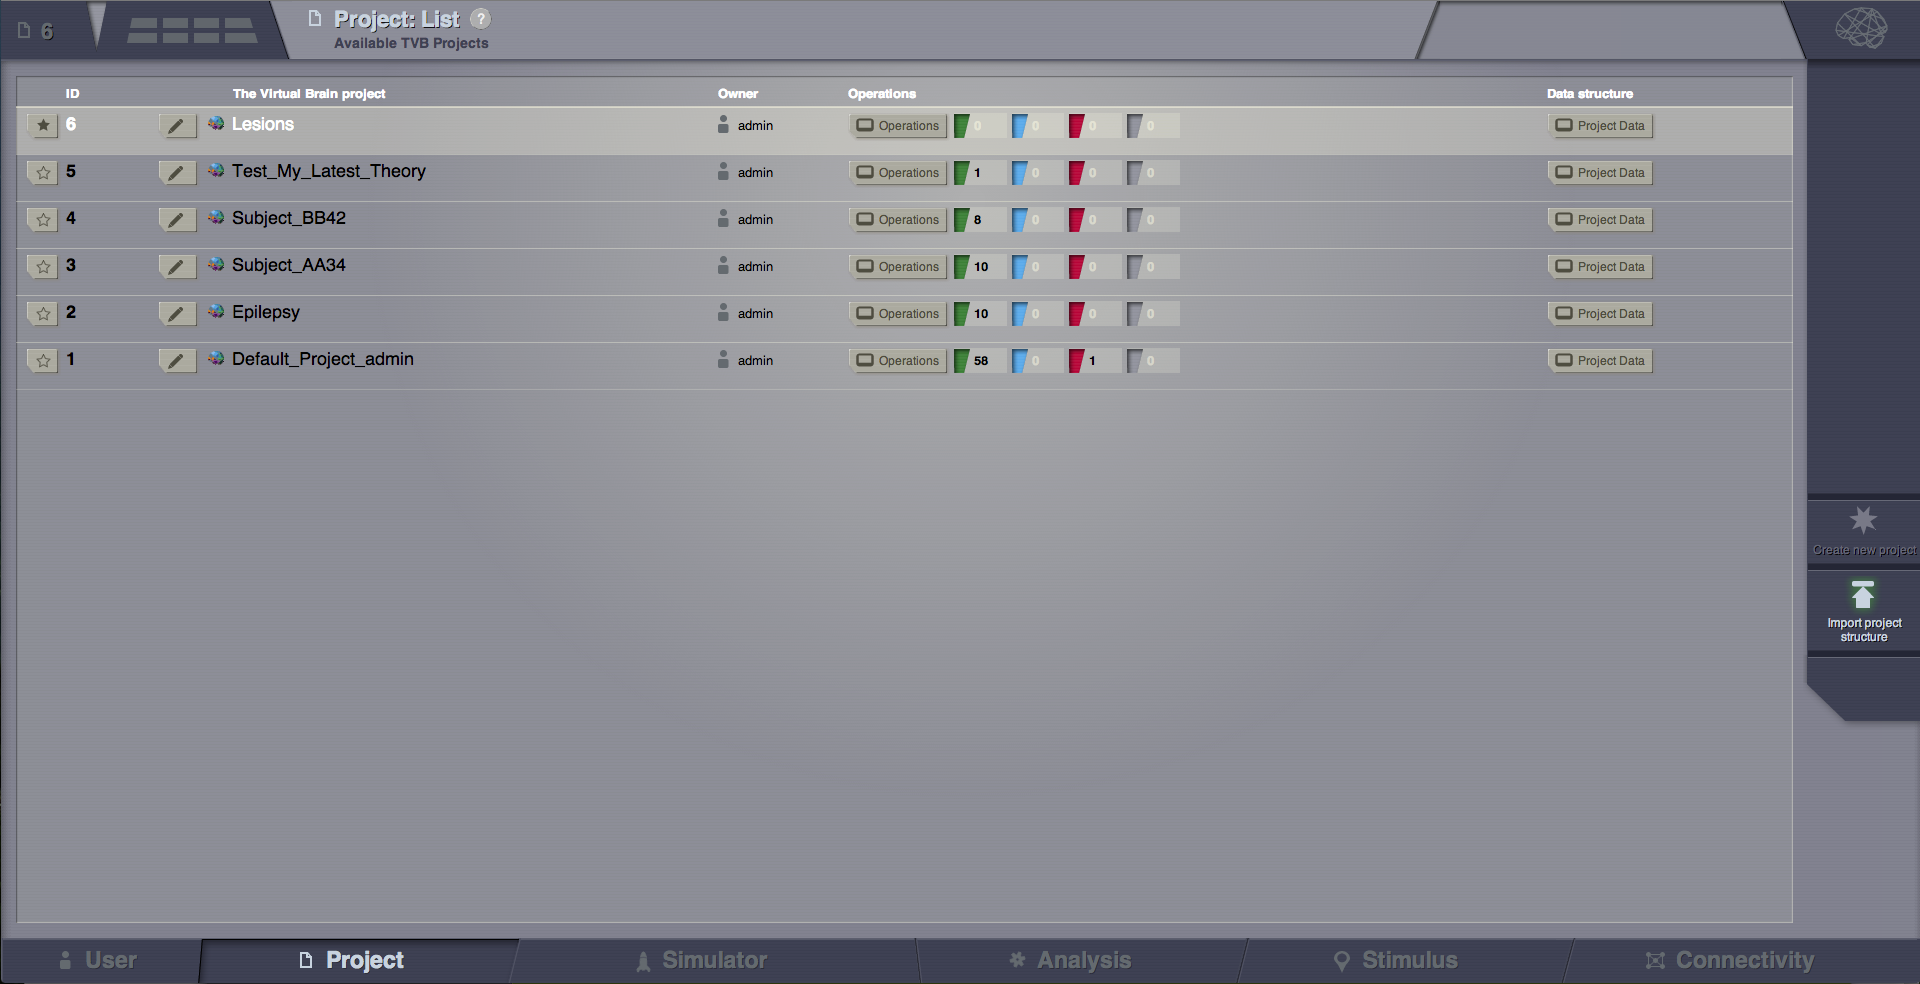
\includegraphics[width=0.47\textwidth]{images/ui_projects.png}}
		\\
		\subfloat[][]{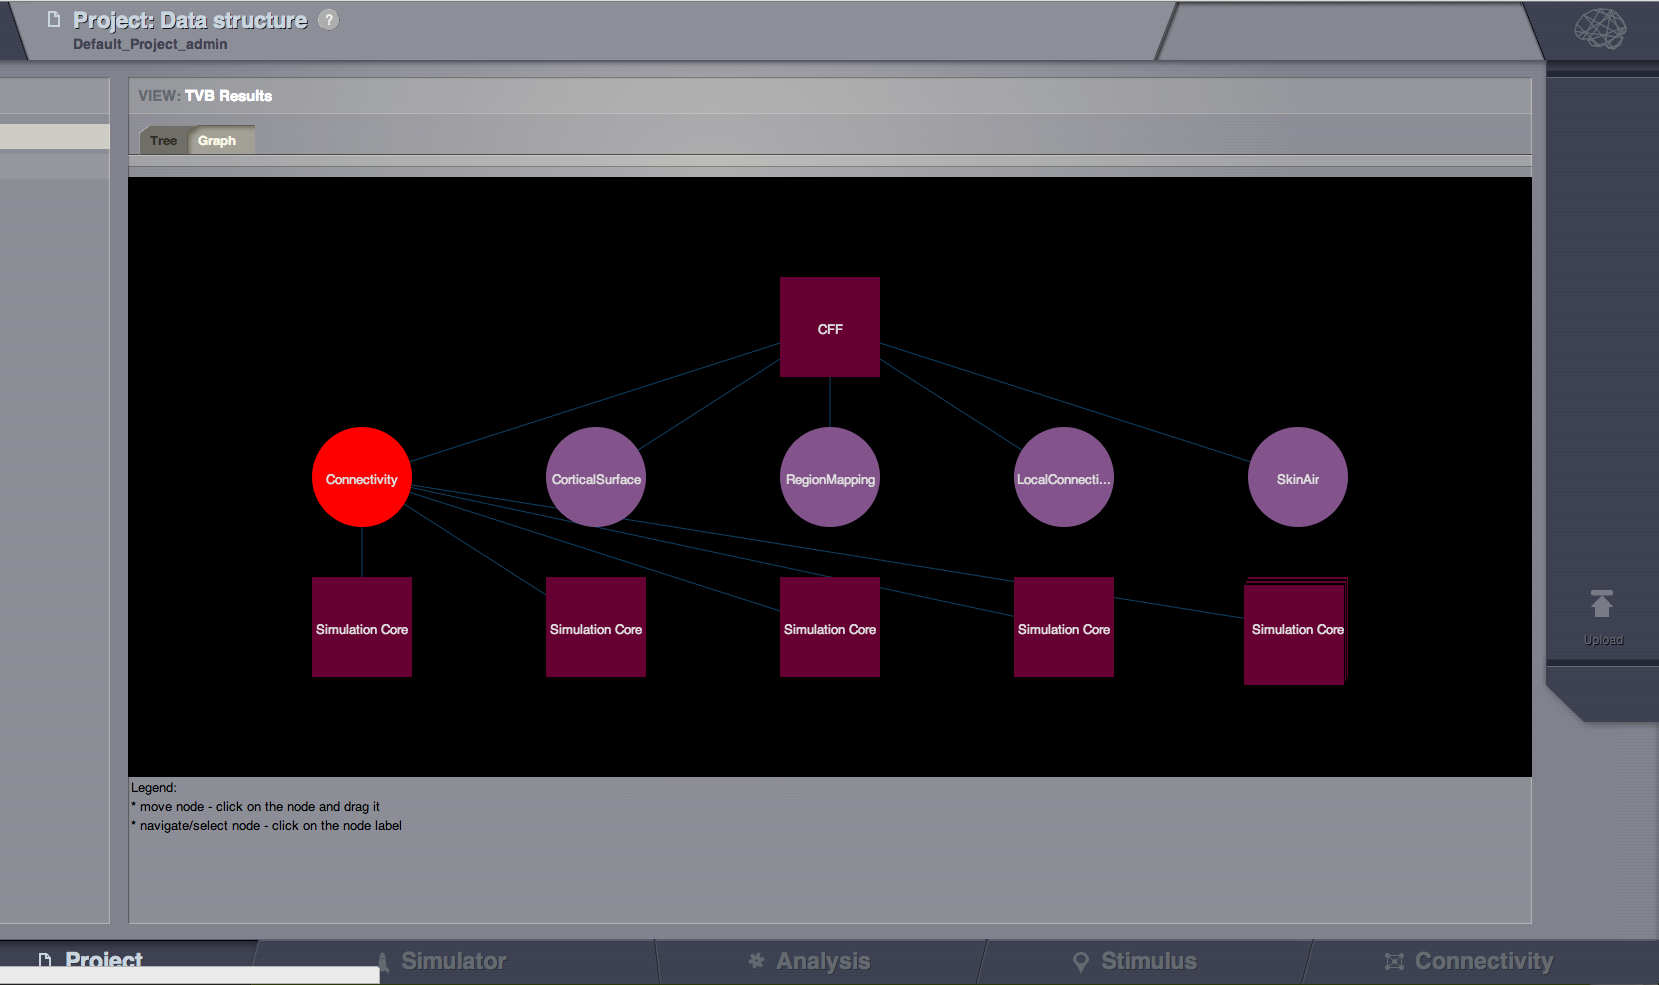
\includegraphics[width=0.47\textwidth]{images/ui_project_graph.png}}
		\\
		\subfloat[][]{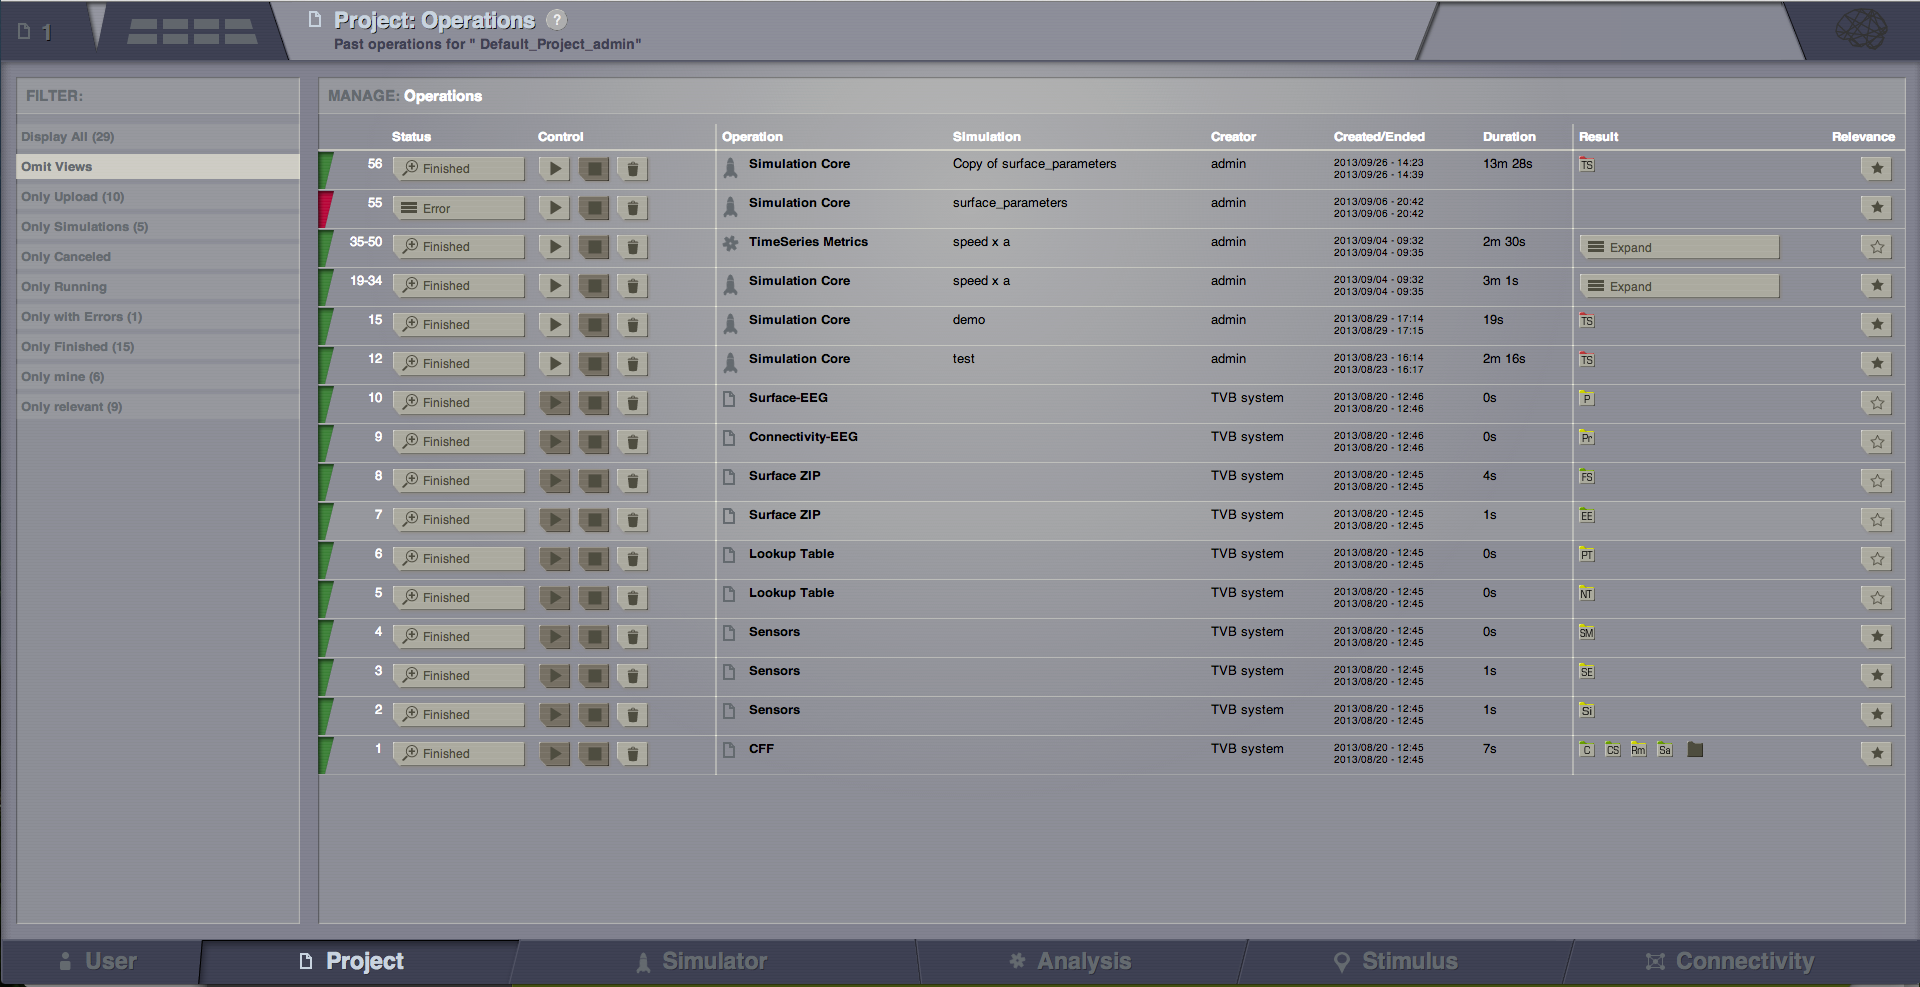
\includegraphics[width=0.47\textwidth]{images/ui_project_operations.png}}
		\\
		\subfloat[][]{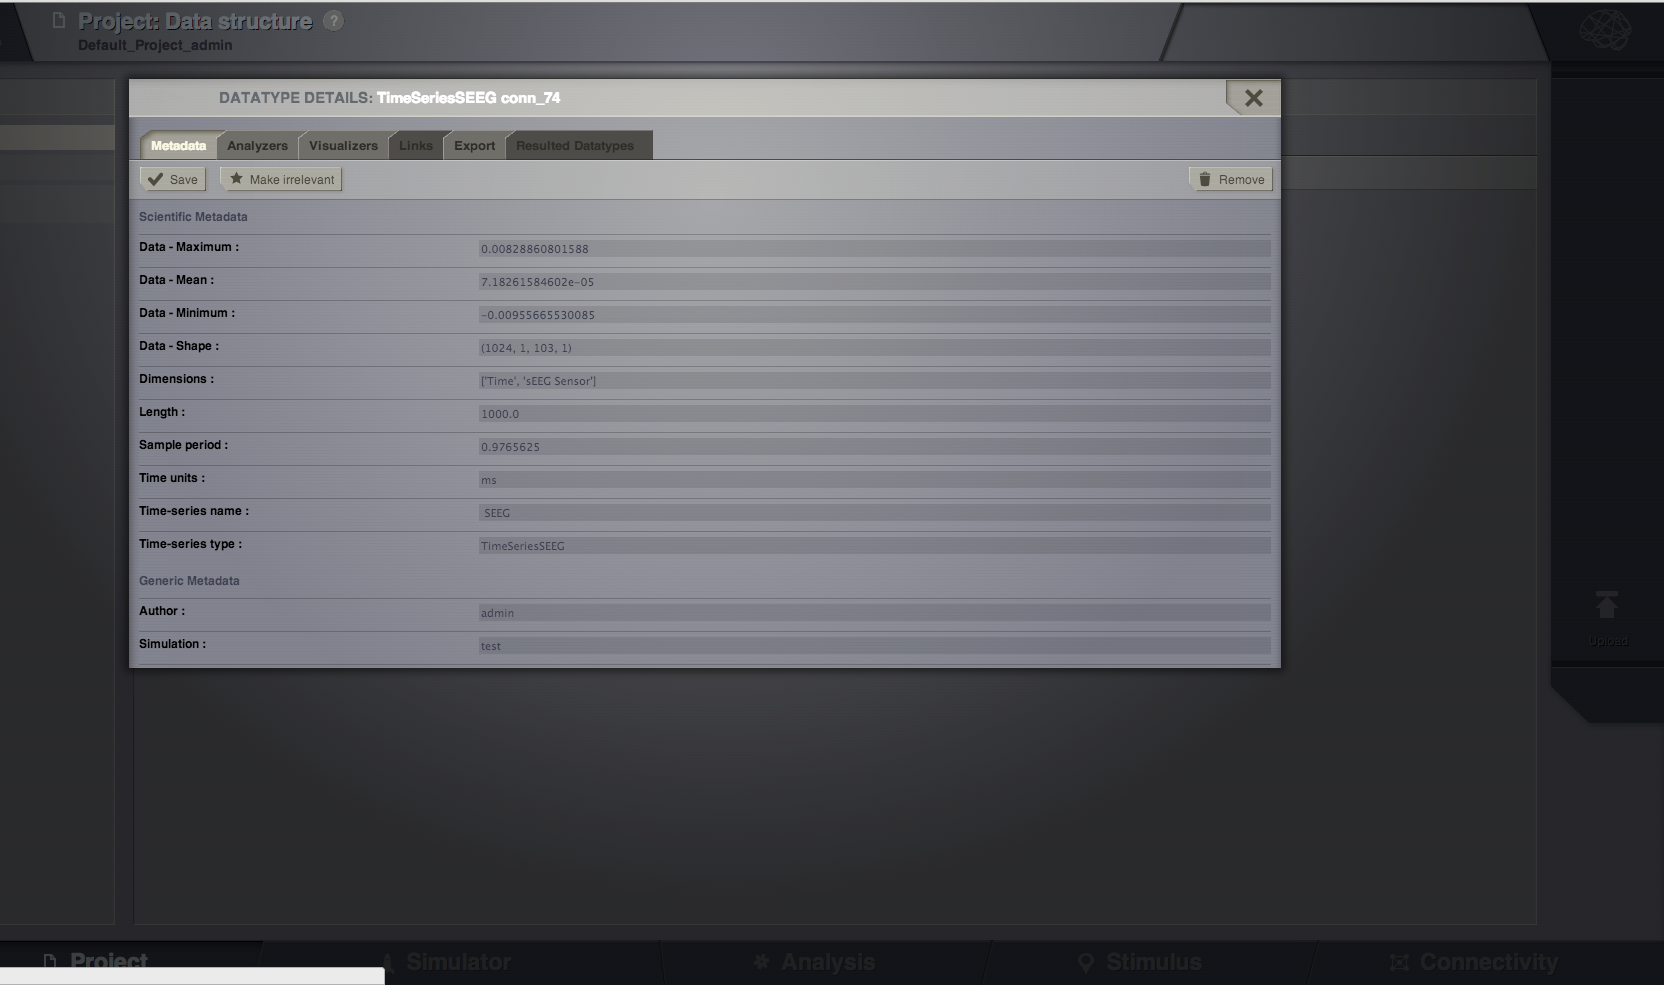
\includegraphics[width=0.47\textwidth]{images/ui_project_datatype_details.png}}
		\caption{\TVB data organization
		(A) View all projects
		(B) 2D graph display of operations with their input and output datatypes 
		(C) View all operations in current project with their status, duration, results, etc
		(D) Datatype details and further available operations for it. This menu becomes available after clicking a datatype result from several places in TVB }
				\label{fig:project}
\end{figure}

		An \emph{Account} or \emph{User} is needed for accessing TVB through
		the web interface.  When TVB web interface is started for the first
		time, the user is requested to provide a username and 
		password for the first account, which acts as an \emph{administrator}.
        Thereafter, others users on the same TVB server can \emph{register}
		for accounts, which are validated by the administrator account.

		A \emph{Project} in TVB is a logical grouping of data and operations: 
        for example, one could choose to
		create a project for each experiment in TVB, while others might
		create projects for each subject of a group. Each project has a single
		user (or account) as owner, but a project may be shared
		with other users to allow for collaboration.

		The execution of an adapter results in an operation, in the
		context of a project. For example, operations are created for each
		simulation, a spectral analysis or surface visualization. 
        Operations have show their status in the user interface, changing from
		\emph{started} to \emph{canceled}, \emph{finished successfully} or
		\emph{finished with error}. 

		A \emph{workflow} in TVB is, conceptually, sequence of operations from simulation,
        through analyses, to visualization(s). A particular workflow applies
		 a default \emph{tag} on the associated operations and
		datatypes.
        The user may also add custom tags to further organize data.

		\subsubsection{Simulator Interface}

		\begin{figure}[!htbp]

		\centering
			\subfloat[][]{\includegraphics[width=0.47\textwidth]{images/ui_simulator.png}}
			\\
			\subfloat[][]{\includegraphics[width=0.47\textwidth]{images/ui_simulator_setup_region.png}}
			\\
			\subfloat[][]{\includegraphics[width=0.47\textwidth]{images/ui_simulator_setup_surface.png}}
			\\
			\subfloat[][]{\includegraphics[width=0.47\textwidth]{images/ui_simulator_setup_region_noise.png}}
			\caption{\TVB Simulator Area: 
                (A) View of the main interface. \textit{Left}, the history column displays the
                information about the simulations and their status; \textit{middle}, the
            simulation column is where simulations are configured,
            change of model, parameters, simulation length; \textit{right}, the
            visualization column, provided configurable, multipanel
            visualizers to display the resulting time series or other visualizers
            that will add an analysis step before displaying the results.  (B)
            Region-based simulation configuration. The parameters of the
            mass model can be set independently for each node.  (C) Surface-based
            simulation configuration, allowing the user to define spatially
            inhomogeneous parameters. (D) Define parameters of the simulation's noise. }
		\label{fig:simulator}
		\end{figure}

		The \emph{Simulator} page is a configurable multicolumn interface 
        that combines TVB simulation, analysis and visualization functionalities (Fig.\ref{fig:simulator} A).

		In the left column, a history of all simulations is kept, allowing
        quick access to previous results and their metadata. Here, the user
        may check metadata, add tags and rename or delete the simulation.

		The middle column of the \emph{Simulator} area is where users configure their
		large-scale brain network model. On the top of this column there is a blank
		field to name each particular configuration and a button to launch simulations.
		Via this column, users have access to all the configurable components that might
		be used in a simulation, namely:

		{\small

		\begin{itemize}
			\item long range connectivity (i.e., the connectome or connectivity matrix);
			\item long range coupling function (to scale the weights in the connectivity matrix);
			\item conduction speed;
			\item cortical surface;
			\begin{itemize}
				\item local connectivity kernel;
				\item local connectivity strength (can be configured to be different for each vertex);
				\item region mapping (correspondences between vertices of the surface and anatomical regions in the connectome);
			\end{itemize}
			\item stimulus
			\item local dynamics model (i.e. neural mass model)
				\begin{itemize}
					\item state variable range;
					\item state variables to be recorded and stored;
					\item initial conditions (seed and type of noise used to set random initial conditions);
				\end{itemize}
			\item integration scheme;
			\begin{itemize}
				\item if stochastic, the random seed can be set as well as the type of noise (white, coloured);
				\item integration time step size;
			\item monitors (you can set the monitors period to downsample the raw time-series)
			\item simulation length
			\end{itemize}
		\end{itemize}
		}

		Additional information about the components (e.g., modules, datatypes
		and their attributes) is available  by clicking on the question
		mark icon next to each element. This documentation is pulled from the
		annotations provided by the traits system and documentation strings.

		Specific pages are accessible for setting up the neural mass model
		parameters in region-based and surface-based simulations, as well as
		for configuring the noise amplitude in stochastic integrations (only
		for region-based simulations) (Figs. \ref{fig:simulator} B, C and D)
		The ``Set up region Model'' area consist of an interactive phase-plane
		display. This tool shows the 2-dimensional planes of the general
		N-dimensional phase space of the local dynamic model. This tool is
		used to observe how the dynamics of the physical model change as a
		function of its parameters, acting as a guide to set those parameters
		appropriately.

		On the right column, different displays can be configured to show 
		the simulated time series and to add an analysis step with a subsequent
        visualization of the
		results, for example, computing the correlation coefficients and visualizing the
		resulting matrix).

        For many of the parameters, such as 
        a parameter of the local dynamics model, coupling
		strength, conduction speed, among others, 
        it is possible to specify a range of evenly
        spaced values, and launch the corresponding sweep in
        parallel, using several CPU cores. When the simulation results
        are available, a common metric, such as average variance or 
        degree of synchronization, is applied to the time series, and a 
        one or two dimensional plot, determined by the number of parameters
        for which parameter ranges were provided, is shown, allowing
        the user to see how the simulation changes with the chosen parameters
		(Fig.\ref{fig:visualizers} D).
		
		\subsubsection{Analysis \& Visualizers}

			TVB does not intend to provide fully featured, complex data analysis
            techniques, which have been well covered by other packages. 
            Instead, we offer a minimal set of standard algorithms to quickly
            validate simulation results or compare with imported patient data; 
            these include principal and independent component analyses, 
            Fourier and wavelet spectral analyses, correlation and coherence
            analyses, and for connectivity, an interface to the Brain 
            Connectivity Toolbox \citep{Rubinov_2010}. 

			For each of the datatypes produced in TVB, one or more
			visualizers are available, each taking advantage of the best
            techniques available:

			 \begin{figure}[!htbp]
					\subfloat[][]{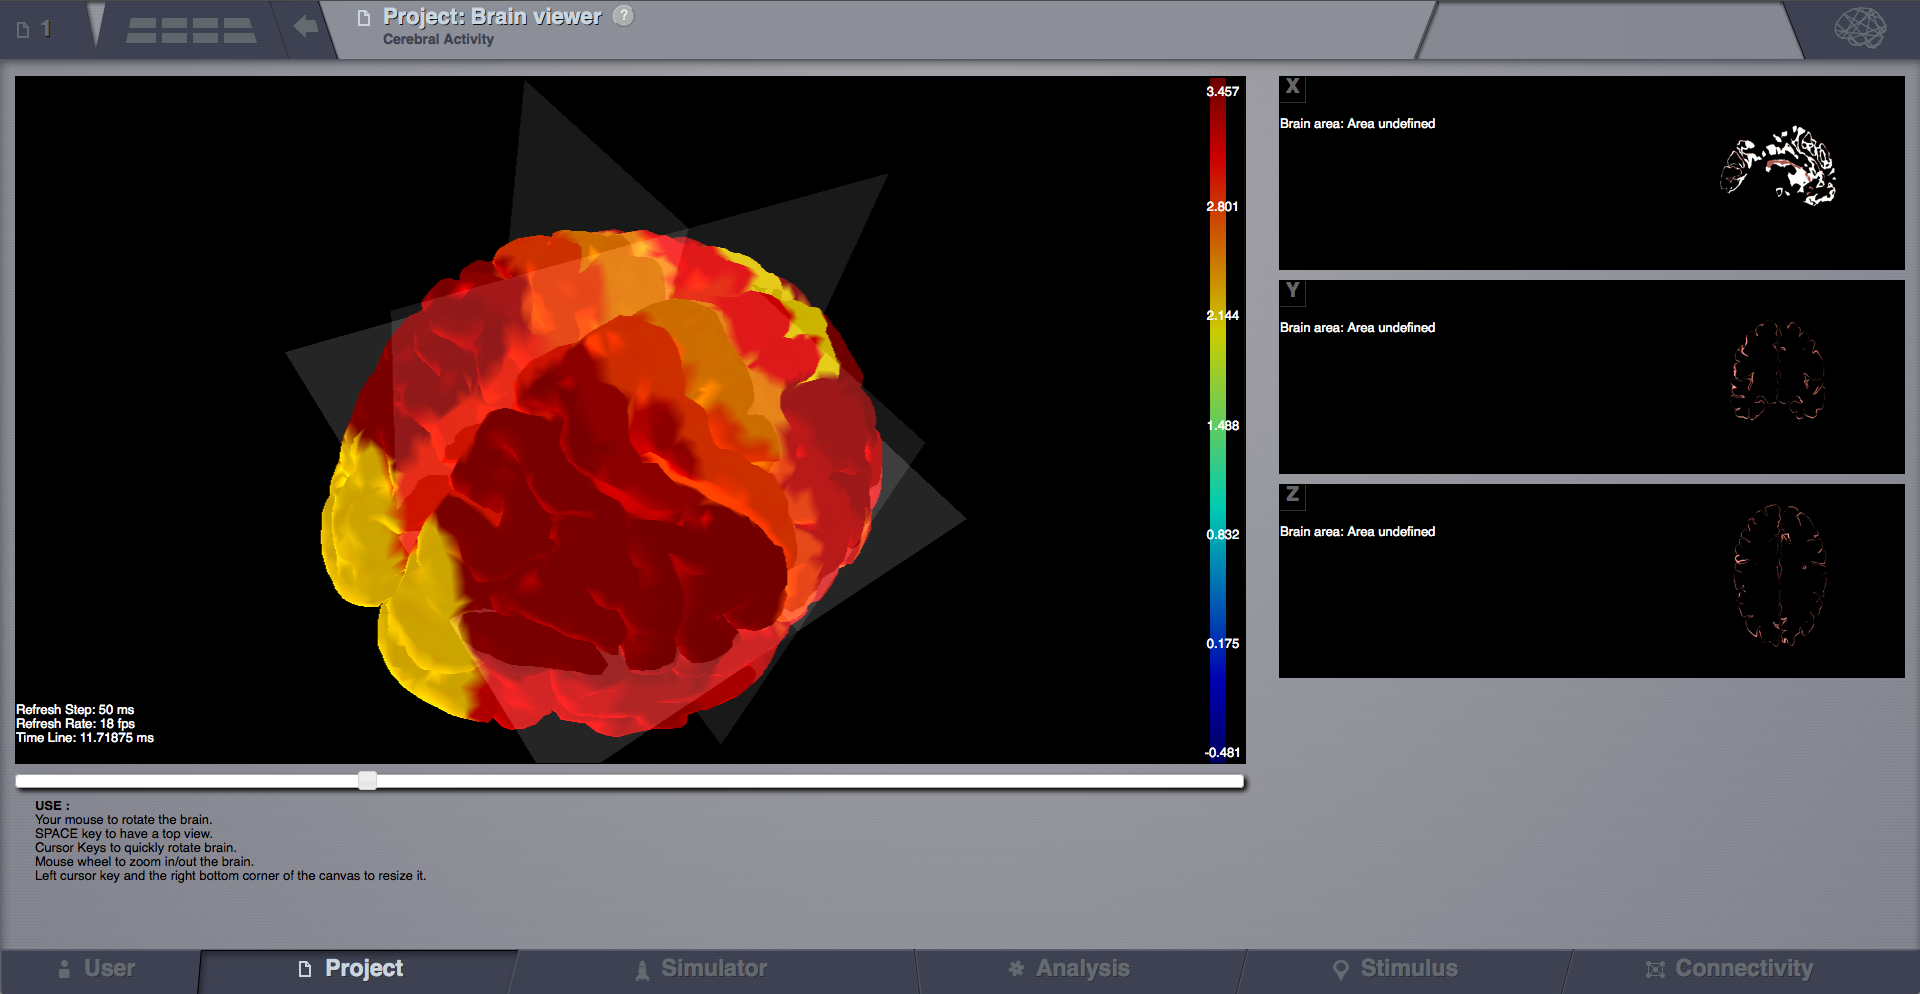
\includegraphics[width=0.48\textwidth]{images/ui_view_brain.png}}
					\\
					\subfloat[][]{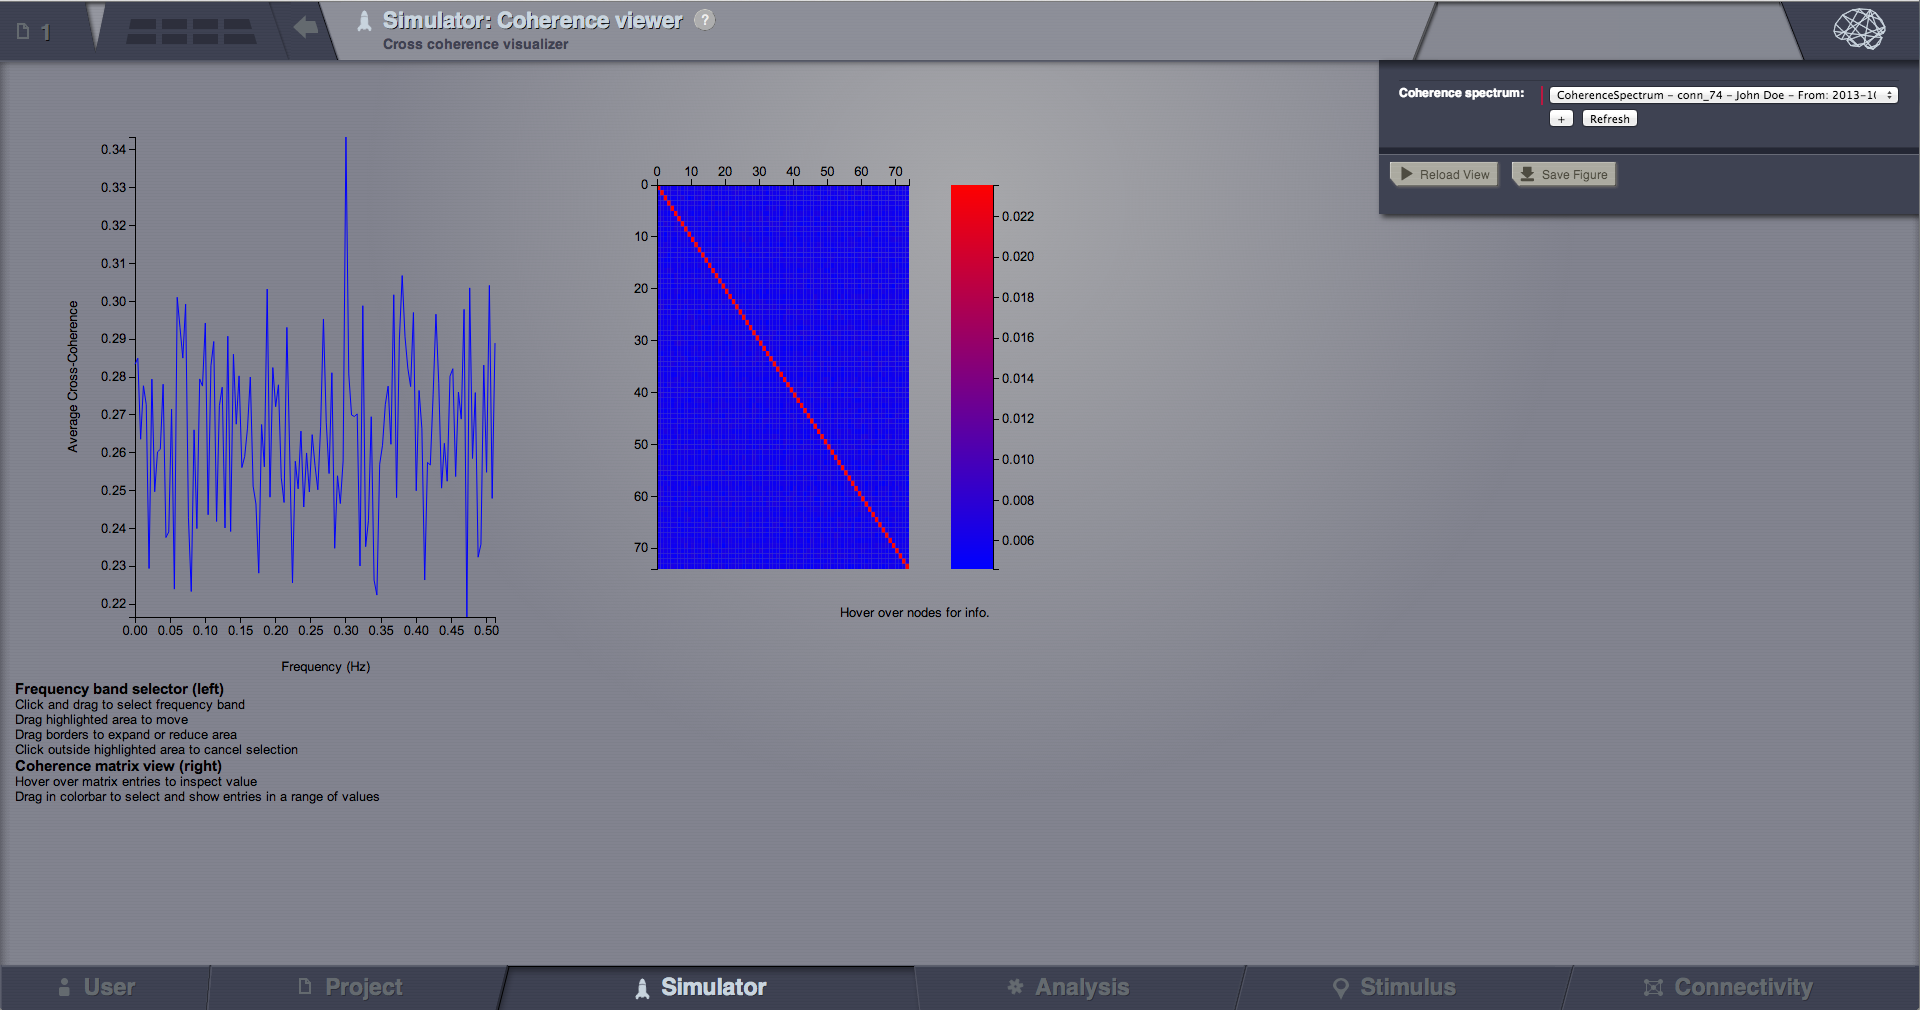
\includegraphics[width=0.48\textwidth]{images/ui_view_coherence.png}}
					\\
					\subfloat[][]{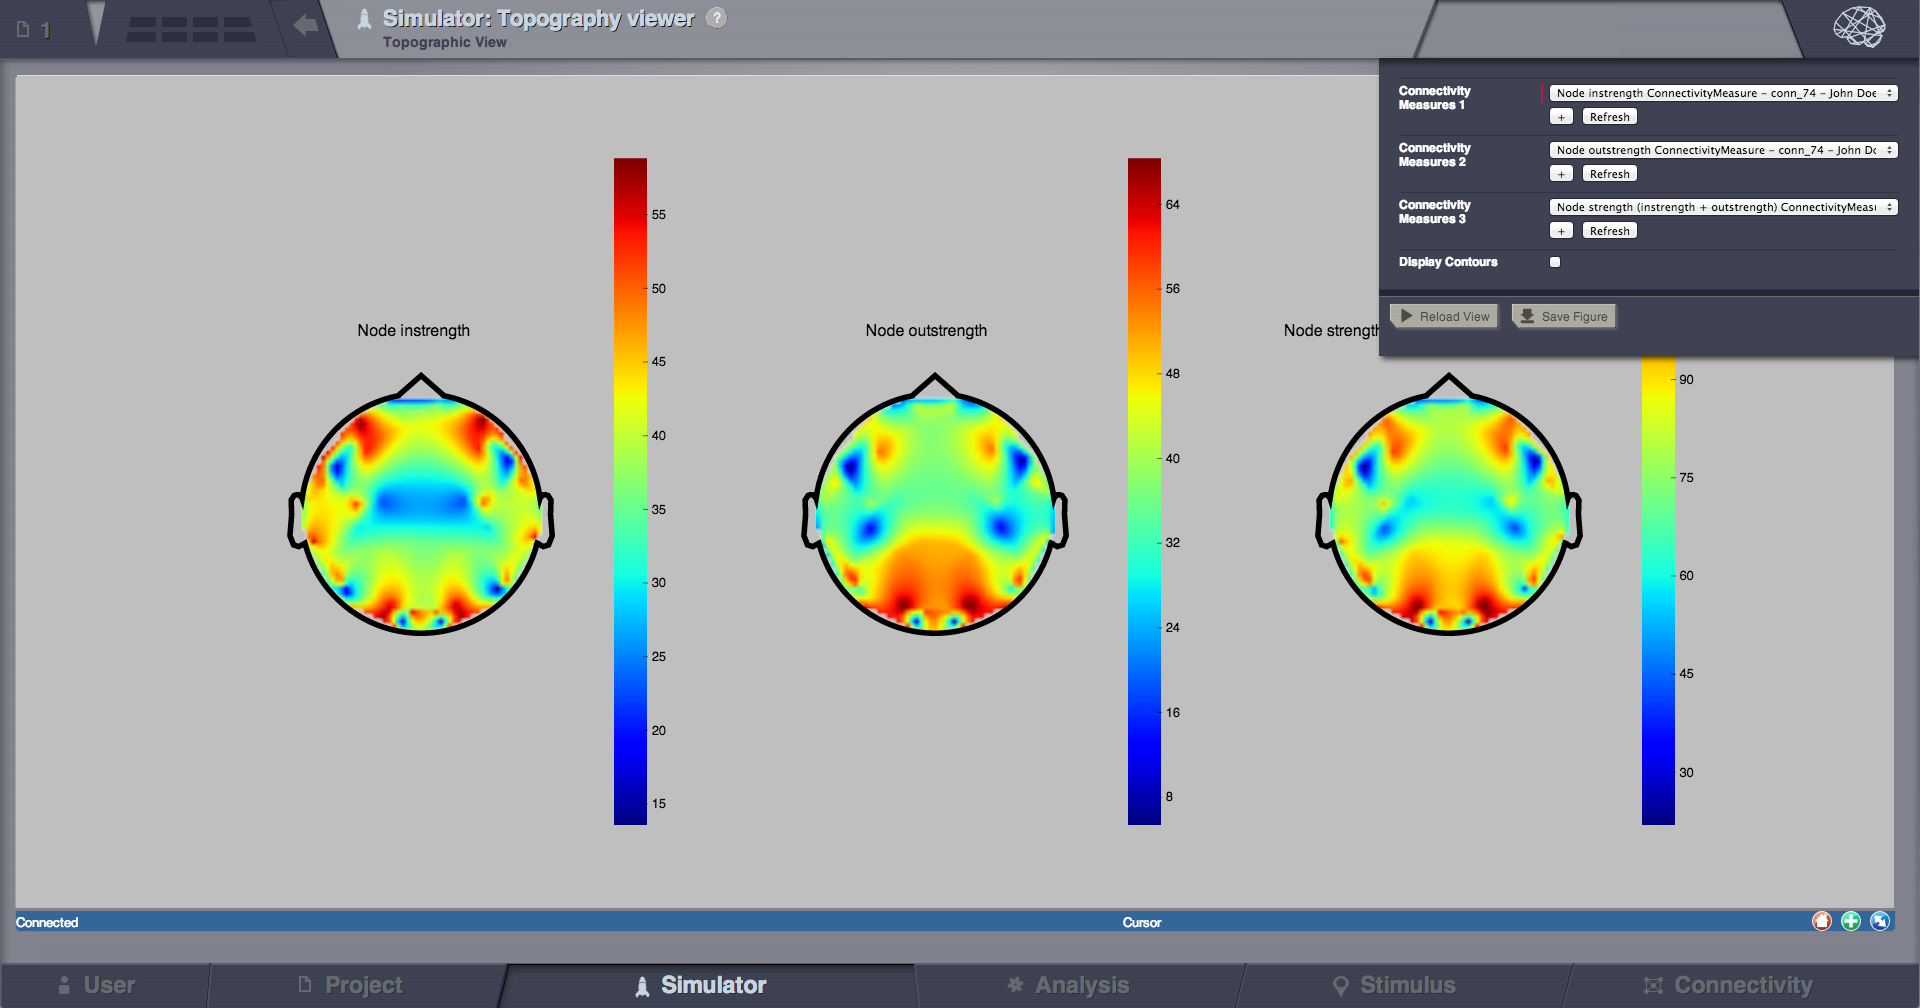
\includegraphics[width=0.48\textwidth]{images/ui_view_topo.png}}
					\\
					\subfloat[][]{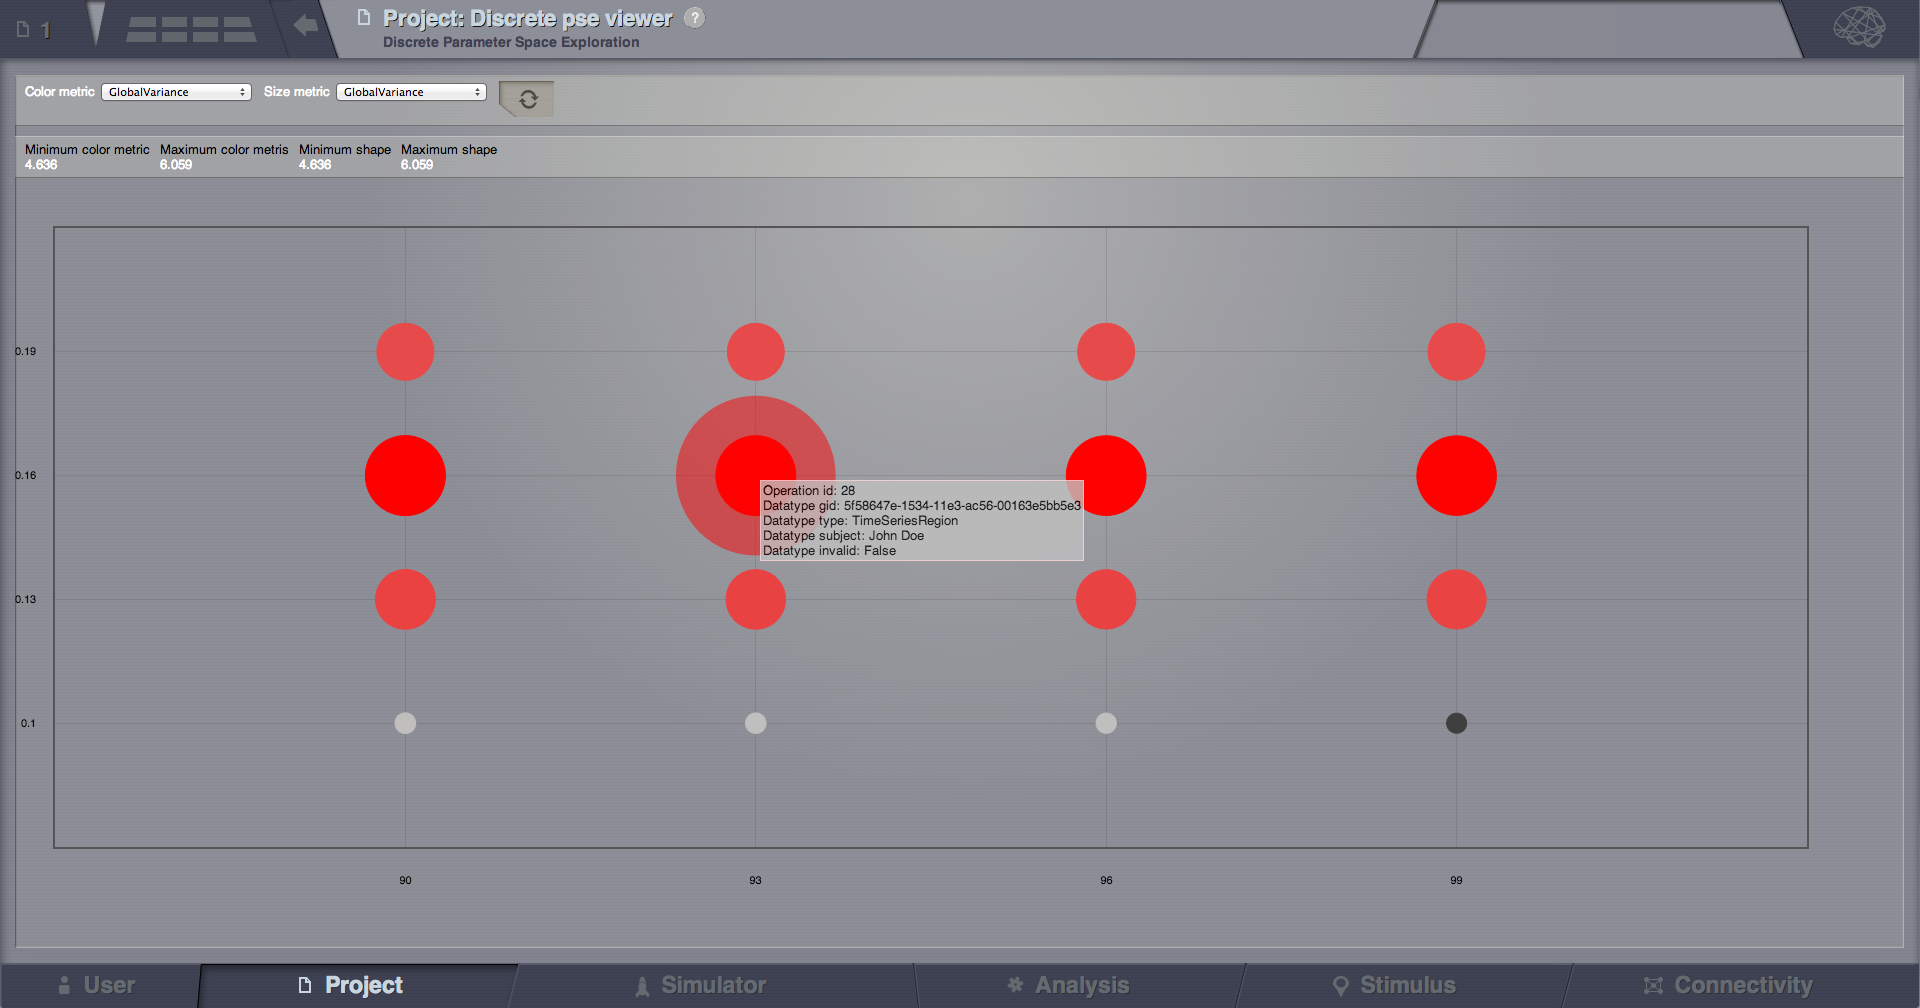
\includegraphics[width=0.48\textwidth]{images/ui_view_pse.png}}
					\caption{\TVB visualizers: 
					(A) WebGL: 3D display of region level simulated signal, mapped on a brain cortical surface
					(B) SVG: Cross Coherence
					(C) MPLH5:  Topographic view with Connectivity in/out strength measures
					(D) FLOT: Parameter Space Exploration results grid}
				\label{fig:visualizers}
			\end{figure}
	
	\begin{enumerate}
		\item \emph{WebGL viewers} are based on \emph{HTML 5 Canvas} element
		and the \emph{gl} context. These viewers offer a 3D display,
		 user interaction with the scene (rotate,
		translate, zoom), and high performance for complex visualizations.
        WebGL is used primarily for visualizing cortical surfaces.
		
		\item \emph{SVG viewers} use a high-quality, highly interactive vectorial 
            format. We
		use such viewers for manipulating and displaying time series,
		covariance or cross coherence datatype results. These visualizers
		were developed specifically for these data types in TVB, and provide a 
		richer level of interaction.

		\item \emph{MPLH5 viewers} use  emph{Matplotlib}'s \emph{HTML 5}
		backend for viewing some of TVB's datatypes, such as
		the Fourier and spectral analyses. 

		\item \emph{Other} simpler viewers in TVB use the JIT
		\url{http://philogb.github.io/jit/} or FLOT
		\url{http://www.flotcharts.org/} Javascript libraries. These are mainly
		2D plots for simple TVB generated data.
	\end{enumerate}

\subsubsection{Connectivity Tools}

		\emph{Connectivity}, in the context of TVB, is another datatype, mapping structural
		information about a subject (a real single individual or an average template). For
		editing and viewing a connectivity, TVB has a dedicated interface, where
		the \emph{G-User} can manipulate connectivity strength and lengths
		at the granularity of individual edges.
        Note that we do not store or use information about the exact anatomical path or
		a connection, only the region centers and connection weights and
		lengths.

 \begin{figure}[!htbp]
		\centering
		\subfloat[][]{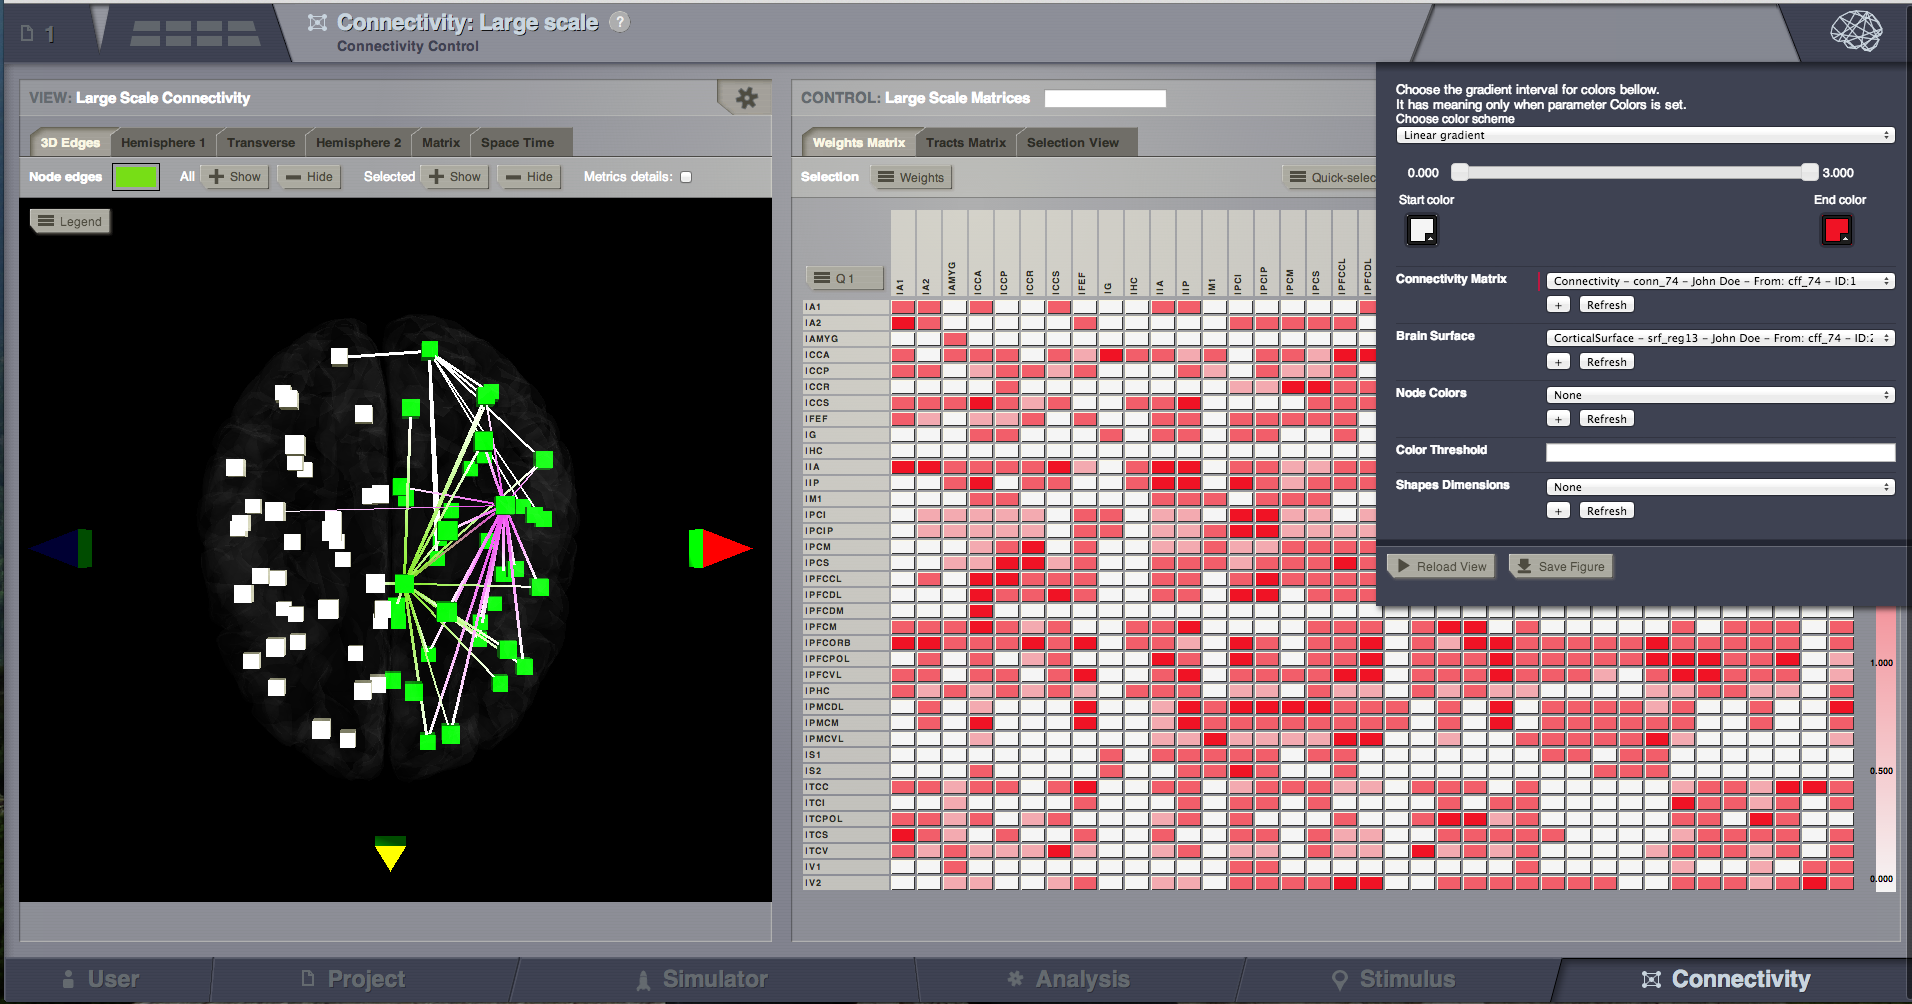
\includegraphics[width=0.48\textwidth]{images/ui_connectivity.png}}
		\\
		\subfloat[][]{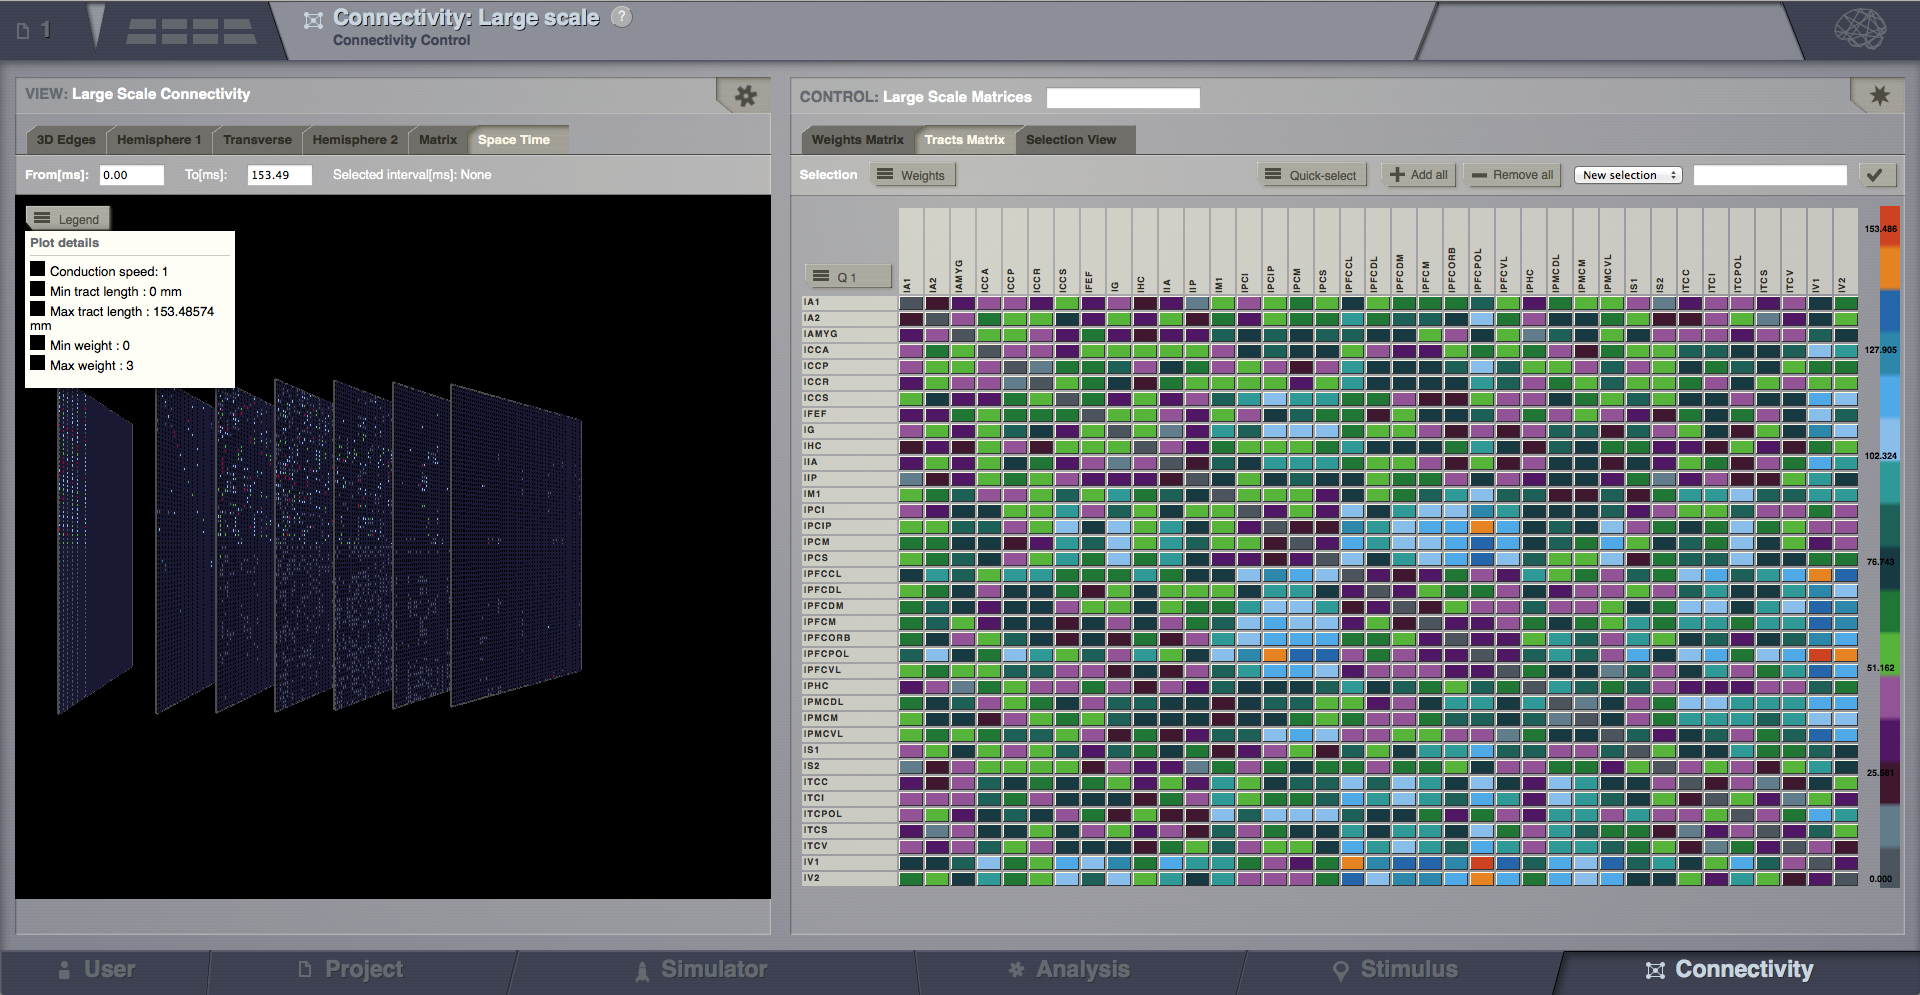
\includegraphics[width=0.48\textwidth]{images/ui_connectivity_delays.png}}
		\caption{Connectivity tools: 
            (A) \textit{Left}: Displaying weighted connections between selection of nodes, with 3D manipulation.
            \textit{Right}: Editing weight connections, one at a time, or many.
            (B) \textit{Left}: Show effect of connectivity delays (in milliseconds) when conduction speed is 1 mm/ms.
        \textit{Right}: Editing and displaying one quadrant from the matrix of connection tracts.}
				\label{fig:connectivity}
\end{figure}

\subsubsection{Stimulus Editor}

    The \emph{Stimulus} interface assists users in generating
	stimulation patterns that maybe be later used in a simulation, for 
    example to model the effects of transcranial magnetic stimulation.
    The way in which stimuli are designed depends on whether the simulation
    will be at region-based or surface-based.
	For region-based simulations, a
	unique temporal profile can be specified for each node, with the amplitude
	of the stimulation modulated individually for each node. For surfaces,
	in addition to the temporal profile, it is possible to select several vertices
	on the surface to define the foci around which the spatial pattern is centered.
    A stimulation profile in TVB is a \emph{pattern}
	datatype, either uniquely temporal or spatiotemporal depending the
	spatial support of the network.

\subsection{Console and scripting}

The components of TVB are of course accessible from a Python
script or, more conveniently, from any of the IPython interfaces.
For example, the tutorials for the simulator have been developed
as IPython notebooks, due to its ability to mix text, mathematics,
code and figures. 

\subsubsection{\texttt{hello\_brain.py}}

To give a basic feel for scripting TVB simulations, we will 
walk through a simple example of a region-level simulation.

\begin{lstlisting}
from tvb.simulator.lab import *
\end{lstlisting}

\noindent which is an all-in-one module making writing scripts
shorter, in the style of \texttt{pylab}, as it imports everything
from \texttt{pylab}, \texttt{numpy} and most of TVB's simulator
modules. Next, we build a simulator object:

\begin{lstlisting}
sim = simulator.Simulator(
    model        = models.Generic2dOscillator(), 
    connectivity = connectivity.Connectivity(),
    coupling     = coupling.Linear(a=1e-2),
    integrator   = integrators.HeunDeterministic(),
    monitors     = (
            monitors.TemporalAverage(), 
    )
)
\end{lstlisting}

\noindent where we've employed a two dimensional oscillator
with default parameters, the default connectivity, a linear 
coupling function with a slope of $1e-2$, and deterministic
Heun integrator and a monitor that temporally averages the 
network dynamics before providing output. Each of these
components can be replaced by a user's subclass of the
appropriate base class, e.g. the value of \texttt{model}
should subclass \texttt{models.Model}.

While TVB strives to keep modules independent of one another,
it is typical for mathematical dependencies to arise between, 
for example, the mass model and the integration time step, so
after configuring a simulator object, it is necessary to invoke

\begin{lstlisting}
sim.configure()
\end{lstlisting}

\noindent which results in walking the tree of objects, checking and 
configuring the constraints among parameters recursively.

The next step is to run through the simulation, collecting
output from the simulator. In this case, it is as simple as

\begin{lstlisting}
ys = array([y for ((t, y),) in  sim(simulation_length=3e2)])
\end{lstlisting}

\noindent where the simulator has been called, returning a 
generator which performs the integration and returns, for each
monitor, the current time and activity. In a case where EEG 
and fMRI monitors, for example, were used, we might write

\begin{lstlisting}
eeg, mri = [], []
for (t_eeg, y_eeg), (t_mri, y_mri) in sim(3e2):
		if y_eeg is not None:
		eeg.append(y_eeg)
		...
\end{lstlisting}

\noindent Because fMRI and EEG monitors have very different
timescales, whenever one monitor return data and the others do
not, the others contain \texttt{None}, hence the check. Building
more complex logic in this loop would permit, for example, online
feedback and modification of connectivity. 

After the simulation loop has finished, you may wish to see the
result, following the previous listing, 

\begin{lstlisting}
plot(ys[:, 0, :, 0], 'k', alpha=0.1)
\end{lstlisting}

\noindent Here we note that \texttt{ys} is four dimensional. The 
simulator has the convention of treating  mass model state as a
three dimensional array of state variables by nodes by statistical
modes. Because \texttt{ys} is an array collected over time, the first
dimension is time, and the plot here is of each node's first state
variable, over time.

Many more demonstrations of the various features of the simulator
can been found in scripts distributed with the sources of TVB, or 
browsed online at \url{https://github.com/the-virtual-brain/scientific_library/tree/trunk/tvb/simulator/demos}.

For more details see the Ipython notebook Tutorial: Anatomy of a Region Simulation 
\url{http://nbviewer.ipython.org/urls/raw.github.com/the-virtual-brain
/scientific_library/trunk/tvb/simulator/doc/tutorials/Tutorial_Anatomy
_Of_A_Region_Simulation/Tutorial_Anatomy_Of_A_Region_Simulation.ipynb}

%\subsection{MATLAB Scripting}

%\input{matlab-ui}


\section{Simulator}
\input{simulator.tex}

\section{Future Work}
\input{future.tex}

\bibliographystyle{apalike}
\bibliography{bib}

\end{document}

